%%==================================================
%% diss.tex for SJTU Master Thesis
%% based on CASthesis
%% modified by wei.jianwen@gmail.com
%% version: 0.3a
%% Encoding: UTF-8
%% last update: Dec 5th, 2010
%%==================================================

% 字号选项: c5size 五号(默认) cs4size 小四
% 双面打印(注意字号设置)
\documentclass[cs4size, a4paper, twoside]{sjtuthesis} 
% 单面打印(注意字号设置)
% \documentclass[cs4size, a4paer, oneside, openany]{sjtuthesis} 


% \usepackage[sectionbib]{chapterbib}%每章都用参考文献
\usepackage{subcaption}
\usepackage{algorithm}  
\usepackage{algorithmic}
\renewcommand{\algorithmicrequire}{ \textbf{Input:}} %Use Input in the format of Algorithm
\renewcommand{\algorithmicensure}{ \textbf{Output:}} %UseOutput in the format of Algorithm
%\usepackage{url}
%\usepackage{href}
%\usepackage{fancyhdr}                                
%\usepackage{lastpage}                                           
%\usepackage{layout} 

\newboolean{DOIT}
\setboolean{DOIT}{false}%编译某些只想自己看的内容,编译true,否则false

%% 行距缩放因子(x倍字号)
\renewcommand{\baselinestretch}{1.25}

% 设置图形文件的搜索路径
\graphicspath{{figure/}{figures/}{logo/}{logos/}{graph/}{graphs}}

%%========================================
%% 在sjtuthesis.cls中定义的有用命令
%%========================================
% \cndash 中文破折号
% 数学常量
% \me 对数常数e
% \mi 虚数单位i
% \mj 虚数单位j
% \dif 直立的微分算符d为直立体。
% 可伸长的数学箭头、等号
% \myRightarrow{}{}
% \myLeftarrow{}{}
% \myBioarrow{}{}
% \myLongEqual{}{}
% 参考文献
% \upcite{} 上标引用
%%========================================


\begin{document}

%%%%%%%%%%%%%%%%%%%%%%%%%%%%%% 
%% 封面
%%%%%%%%%%%%%%%%%%%%%%%%%%%%%% 

% 中文封面内容(关注内容而不是形式)
\title{混合现实眼镜的交互设计与应用研究}
\author{何贞毅}
\studentnumber{1120379035}
\advisor{杨旭波教授}
%\secondadvisor{教授}
\degree{工程硕士}
\major{软件工程}
\institute{软件学院}
\defenddate{2015年1月}
\school{上海交通大学}

% 英文封面内容(关注内容而不是表现形式)
\englishtitle{INTERACTION DESIGN AND APPLICATION STUDY WITH MIXED REALITY GLASSES}
\englishauthor{\textsc{Zhenyi He}}
\englishadvisor{Prof. \textsc{Xubo Yang}}
%\englishassistadvisor{Prof.}
\englishdegree{Master of Engineering}
\englishmajor{Software Engineering}
%\englishinstitution{School of Software}
\englishdate{Jan. 2015}
\englishschool{Shanghai Jiao Tong University}
%\englishinstitution{\textsc{School of Software} %\\
  %\textsc{Shanghai Jiao Tong University} \\
  %\textsc{Shanghai, P.R.China}
  %}


% 封面
\maketitle

% 英文封面
\makeenglishtitle

% 论文原创性声明和使用授权
\makeDeclareOriginal
\makeDeclareAuthorization

%%%%%%%%%%%%%%%%%%%%%%%%%%%%%% 
%% 前言
%%%%%%%%%%%%%%%%%%%%%%%%%%%%%% 
\frontmatter

% 摘要
%%==================================================
%% abstract.tex for SJTU Master Thesis
%% based on CASthesis
%% modified by wei.jianwen@gmail.com
%% version: 0.3a
%% Encoding: UTF-8
%% last update: Dec 5th, 2010
%%==================================================

\begin{abstract}
近些年来,越来越多的混合现实设备被研制出来,不论是手持式还是佩戴式都层出不穷,而对于其交互手段、交互界面与应用场景均尚在探索阶段。
其中混合现实设备上的交互界面仍以二维界面为主,虽然简洁明晰但却与用户所处的三维空间不相符合;
此外,对于此类设备的交互手段研究相当丰富,一部分以肢体、声音及触觉等人体感知的方法进行交互,另一部分设计出增强媒介如带有图案(pattern)的笔等来进行交互,
方式不同而关键在于是否适合所设计的应用环境及用户体验是否良好;
多数增强与混合现实应用都具有导入模型的功能,导入模型虽然方便却不具有个性化,
针对用户在增强与混合现实的应用场景下进行模型创建的研究也很多,如何避免用户自身的建模能力不足又同时赋予用户足够的自由度则是主要的难点。
本文围绕这些问题,主要针对(1)混合现实眼镜的制作;(2)三维交互界面;(3)以手势为主的交互手段;以及(4)应用性广泛的徒手三维建模场景进行设计与评估。

本文完成的主要工作成果有:

(1)首先制作一个视频透视的混合现实眼镜,为之后的研究工作做铺垫。

(2)在自制的混合现实眼镜下设计了调色盘菜单,并针对不同的思维模式设计了三种布局,分别是手掌召唤式菜单、目标跟踪式菜单及屏幕固定式菜单。

(3)针对虚拟物体的基本操控设计了以手势为主配合头部动作的交互方式,并为了用户更好的体验增加了头部约束、骨骼小球和顶置提示板作为辅助功能帮助用户交互。

(4)针对增强与混合现实应用中常用的模型使用,设计其独特的建模方式,利用该自制设备释放双手的特性,并参考双手交互的三项原则,且针对前人工作中存在的不足提出了改进方法,包括对用户自身建模能力的优化、支持无缝衔接建模时不同状态的切换,和提高用户创建定制模型的自由度,设计并实现了徒手三维建模的应用场景。

每一部分的工作都通过详细的用户实验进行评估,分别验证三维界面、三维操控与徒手三维建模的可行性与易用性。
从用户的反馈与记录的数据中可以初步得出结论,本工作设计的调色盘菜单与基于手势的交互可以应用在眼镜类的混合现实设备上,并且徒手三维建模的应用场景完成度与可用性都较好。

  \keywords{
  %\large 
  \songti\zihao{-4} 混合现实眼镜,手势交互,三维建模,三维菜单}
\end{abstract}

\begin{englishabstract}

In recent years, more and more Mixed Reality(MR) devices were developed, no matter hand-held devices or wearable devices.
While when it comes to the interactive styles, user interfaces and applications of these devices, the researches are still ongoing.
The user interfaces of MR devices are still 2D for most. Although it's clear and simple, it doesn't match the 3D space where users are;
In addition, there are plenty of researches on interaction styles of these devices. Some of them interact through body, audio, tactile sensation and other human sense, while others are based on Augmented Reality(AR) agent like pen with pattern.
The methods are all different, and what matters is whether it's suitable to application and the user experience.
Apart from that, many AR and MR application has the function of importing models.
It's convenient to import models, but it's not personalize.
There are many researches on creating models in AR and MR application either.
The main difficulties are how to avoid the shortness of people's modeling ability and how to maximize people's freedom to create.
This work focused on these problem:
(1)the fabrication of a MR glasses,
(2)the 3D user interface,
(3)the user interaction style based on gestures,
and (4)3D modeling with bare hands, which is widely used in applications.
Evaluation are presented after design.

The followings are main work in this paper:

(1)First, a video see-through MR glasses is made by ourselves, which is used for the rest of our work.

(2)Palette-like 3D menus and three kinds of placement are designed and implemented based on MR glasses to meet different ways of thinking, such as palm-based menus, object-tracked menus and screen-fixed menus.

(3)3D basic manipulation method mainly based on gestures are designed and implemented, and head motion is supported for assistance.
In addition, to improve the user experience, different assistance methods including head constraints, skeleton balls and board are added to support user's manipulation.

(4)At last, a new method of creating 3D models, which is familiar in all kinds of AR and MR applications is presented.
We created our own principles for bimanual interaction on 3D modelling based on the hands-free devices and former principles
and the 3D modeling application with bare hands.
We pinpoint the shortage of previous work and improve people's modelling result even they are bad model creators by a seamless modelling environment among different status switch, and enough freedom for people to create their own models. 

After all, we evaluate the feasibility and usability of every part of the work by experiments, which includes user interface, manipulation and 3D modelling.
We could safely draw the conclusion on user's feedback and data collected in experiments that the palette-like menus and interactive styles for manipulation are suitable under MR glasses, and the application of 3D modelling by two bare hands has got nice feedback as well.

  \englishkeywords{\large Mixed Reality glasses, gesture interaction, 3D modeling, 3D menus}
\end{englishabstract}


% 目录
\tableofcontents
% 插图索引
\listoffigures
\addcontentsline{toc}{chapter}{\listfigurename} %将图索引加入全文目录
% 表格索引
\listoftables
\addcontentsline{toc}{chapter}{\listtablename}  %将表格索引加入全文目录

% 主要符号、缩略词对照表
%%%==================================================
%% symbol.tex for SJTU Master Thesis
%% based on CASthesis
%% modified by wei.jianwen@gmail.com
%% version: 0.3a
%% Encoding: UTF-8
%% last update: Dec 5th, 2010
%%==================================================

\chapter{主要符号对照表}
\label{chap:symb}
\begin{tabular}{ll}

 \hspace{2em}$\epsilon$       & \hspace{5em}介电常数 \\
 \hspace{2em}$\mu$ \qquad     & \hspace{5em}磁导率 \\
  \hspace{2em}$\epsilon$       & \hspace{5em}介电常数 \\
 \hspace{2em}$\mu$ \qquad     & \hspace{5em}磁导率 \\
 \hspace{2em}$\epsilon$       & \hspace{5em}介电常数 \\
 \hspace{2em}$\mu$ \qquad     & \hspace{5em}磁导率 \\
 \hspace{2em}$\epsilon$       & \hspace{5em}介电常数 \\
 \hspace{2em}$\mu$ \qquad     & \hspace{5em}磁导率 \\


\end{tabular}


%%%%%%%%%%%%%%%%%%%%%%%%%%%%%% 
%% 正文
%%%%%%%%%%%%%%%%%%%%%%%%%%%%%% 
\mainmatter


%% 各章正文内容
%%==========================
%% chapter01.tex for SJTU Master Thesis
%% based on CASthesis
%% modified by wei.jianwen@gmail.com
%% version: 0.3a
%% Encoding: UTF-8
%% last update: Dec 5th, 2010
%%==================================================

%\bibliographystyle{sjtu2} %[此处用于每章都生产参考文献]
\chapter{绪论}
\label{chap:what}

\section{研究背景}

%\begin{figure}[!htp]
  %\centering
  %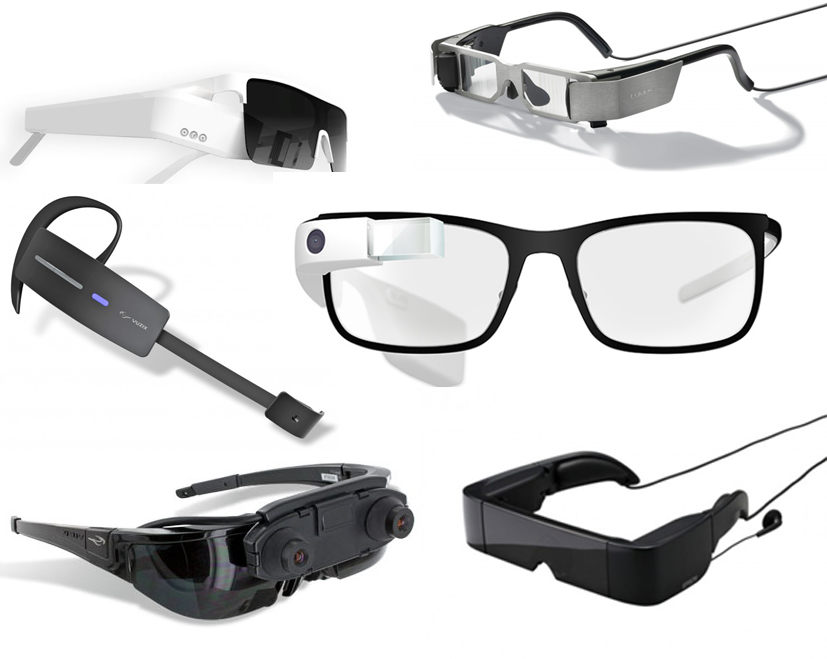
\includegraphics[width=0.8\textwidth]{chap1/ARGlasses}
  %\bicaption[fig:glasses]{增强现实设备}{增强现实设备}{Fig.}{Augmented Reality devices}
%\end{figure}

增强现实(Augmented Reality)是一种将虚拟场景融合进真实场景的技术,其中包括虚拟物体与现实的结合、即时互动以及三维的特性。
增强现实技术可以提供现实中无法获取的信息,用户通过附加的虚拟信息提升对现实场景的了解,增强现实技术在医疗、工业、娱乐与教育上都有广泛的应用前景。
Azuma等人在1997年和2001年\upcite{azuma1997survey,azuma2001recent}及Feng Zhou等人\upcite{FengZhou:2008:TAR:1605298.1605333}在2008年综述了增强现实所需的环境设置、追踪技术、交互技术、用户界面、显示技术及应用发展趋势。

而混合现实(Mixed Reality)则是介于虚拟场景和真实场景之间的一种形态,从图\ref{fig:mr}中看到Milgram\upcite{Milgram:2009:TDC:1643928.1643932}对混合现实,虚拟现实以及真实场景的渐变过程划分,混合现实包含了增强现实与虚拟现实。

\begin{figure}[!htp]
  \centering
  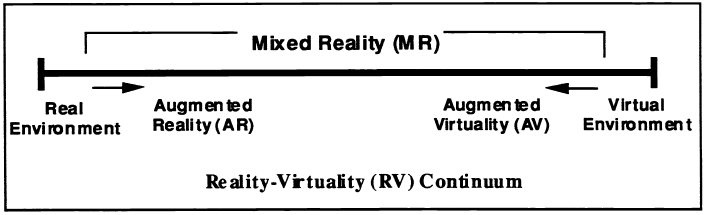
\includegraphics[width=0.95\textwidth]{chap1/Milgram_Continuum}
  \bicaption[fig:mr]{混合现实}{混合现实\upcite{milgram1995augmented}}{Fig.}{Mixed Reality\upcite{milgram1995augmented}}
\end{figure}

随着Google Glass\upcite{googleglass}的上市,智能眼镜成了2014年增强现实与混合现实领域最期待的设备之一。
%,从图\ref{fig:glasses}可见现在炙手可热的一批增强现实穿戴式设备。
眼镜最大的特征在于不需要用户手持进行操作,这一点诸如手机、平板或者更为累赘的台式机、笔记本是完全无法比拟的。
并且眼镜的视野十分宽阔,基本可以覆盖人眼的整个视野,虽然现在的手机越做越大,平板的普及性也很高,但是用户依然可以感受到这些智能设备的边界,而眼镜,就没有这样的局限性。
因而针对眼镜此类设备的研究及其与增强和混合现实应用的结合正是近些年来的研究热点。

针对不一样的设备,关于多点触控、手势、语音控制等多种交互通道的研究层出不穷。
一种类型的交互系统使用单一的通道进行交互,比如平板电脑上的多点触控,或者使用摄像头进行手势识别,再有些利用遥感等传感器进行不同指令的发送。
考虑到视觉通常会受到外界不相干信息干扰,语音控制也是非常直观的一种方式。
另一种类型的交互系统则综合多种通道协作进行交互,诸如利用压力传感,电流反馈等释放双眼、双手的交互方式。
%尽管手势交互因其直观在交互手段中占据了大部分应用,但多种交互手段的尝试对本文的研究是很有必要的。

除了交互手段对增强和混合现实应用有着举足轻重的影响以外,如何在不同的状态间切换、如何区分不同的状态,虽然是一个应用细节,却也极大地影响用户的使用体验。
同样的情形如果在桌面应用上,可能就是一个鼠标点击的区别,即便是最糟糕的情况也莫过于切换过于频繁,让用户很难继续之前的任务。

但在增强现实和混合现实的应用环境下,整个工作环境与输入空间都不是严格固定的,诸如最基本的拖拽还是单纯的移动都无法直接识别,需要通过其他的辅助或者设定才可以完成,因而对于不同交互手段如何在状态间切换也是一个研究热点。
目前状态切换存在着容易混淆\upcite{TrackingBased}、呈现不自然\upcite{Selection}及增加记忆负担\upcite{SideBySide}等问题,值得进一步研究。

与此同时,在对增强和混合现实应用的调研中发现,多数应用都涵盖模型的使用,而关于这点通常都以导入模型来处理。
导入模型虽然简单易行但受控于应用自身的数据库,而且用户无法根据自己的想法创建自定义的符合当前场景的模型。
针对三维建模这一应用场景,现下已经有很多相关的轻量级软件,可以通过简单的操作构建出复杂又美观的模型来。
但在增强和混合现实的应用条件下,哪些设计可以保留并提升,哪些需要舍弃则是另一个需要进一步探索的研究点。
因而需要对物体创建应用在不同的平台如桌面应用、手持移动设备和释放双手的穿戴设备做调研。

桌面应用普遍基于单击工具完成,如Google Sketch\upcite{sketchup}和TinkerCAD\upcite{tinkercad},对于工具的设计是一个很好的切入点。
而其他手持设备在基于单手操作的限定条件下对建模应用进行的设计就非常值得借鉴,比如指尖绘制,通过自制的标签笔进行绘制等,还有释放双手的场景中结合三维场景和平板同时进行模型设计的方法。
其中对于用户建模的难点主要集中在(1)如何克服用户自身不同的绘制水平,帮助用户改善自己的模型。(2)如何提供用户足够的自由度创建有自己特色的模型,不受限于应用的约束。

\section{研究目的}
\label{sec:xulun-mudi}
通过上述对当前背景的了解,本文的研究目的为自行制作一个混合现实眼镜、探索混合现实眼镜设备下直观的交互界面、研究便捷的交互方式及合适的三维建模方式。
为了更清楚地说明自制的混合现实眼镜上的交互界面与交互手段的设计,首先对相关设备、交互、建模和状态切换的研究现状进行详细阐述。
%本文旨在自制的混合现实眼镜上,研究适合此类随身携带的头戴式设备的交互系统,包括交互界面、交互方式及其他辅助方法,让用户使用该系统进行空间设计。
本文将总结研究现状的优点与不足,设计新的三维界面和操控方式,并在此基础上设计新的空间设计方法。
其中交互界面是新设计的一种三维界面,交互方式则是以手势输入为主,配合头部动作形成的多通道交互方式,以此来改善用户体验。
而空间设计方法则是针对三维建模的应用环境,辅助用户制作特制且优质的模型的三维建模方法。

\section{研究现状}
\label{sec:related-cur}
\subsection{光学透视与视频透视}
\label{sec:related-vst}
本文工作的整体实现需要依赖一个便捷的混合现实设备,眼镜。因而对于眼镜的种类及制作方式的调研为一切之基础。混合现实眼镜有两种制作方案,一种是光学透视式,用户透过眼镜镜片观察到真实世界,同时镜片上通过投影或其他方式实现虚拟场景的显示;另一种是视频透视式,镜片即显示器,用户通过镜片观察到已经将真实场景和虚拟场景融合的增强现实结果。FIGI\upcite{FIGI}在光学透视眼镜上无缝连接了数据手套操控和键鼠操控;Mime\upcite{MIME}则通过光学透视眼镜与TOF的结合进行了单手指尖识别。
与之相对,Ha等人\upcite{ha2006bare}通过视频透视眼镜对裸手进行分析与识别;
Looser等人\upcite{LookingGlass}通过视频透视眼镜对现场环境进行识别与操控。
光学透视眼镜在分辨率和视点无偏差上有着优势,但考虑到增强与混合现实应用中经常需要处理的真实物体与虚拟物体间的遮挡,和不同光线下光学透视眼镜受到的影响,本文最终决定通过一个视频透视眼镜来完成眼镜设备上的交互设计与菜单研究。

\subsection{增强现实与混合现实设备上的交互技术}
\label{sec:related-jiaohu}
为了决定在自制的混合现实眼镜下使用何种或者结合哪几类交互手段,本文对增强现实与混合现实设备上的交互方式做了深入的调研与分析。
最通俗常见的是手势交互,为了检测与追踪手部,一部分设备在制作上和交互方式上进行了专门的设计。
SideBySide\upcite{SideBySide}是一套手持相机投影仪套装,通过投影出来的不同影像进行交互,使用过程中使用者总是要被占用掉一只手是最大的不便。
Oakley和Park的工作\upcite{Pointing}通过对手持设备的甩动来进行交互,同样也有这个特点。
王晓春等人\upcite{王晓春2007基于笔交互的表格制作}以及H{\"u}rst等人的工作\upcite{TrackingBased}都设计了一个工具让用户手持进行交互。
王晓春等人\upcite{王晓春2007基于笔交互的表格制作}设计了基于笔的交互,通过对草图的字线分离实现了一种灵活的表格制作方法,在徒手绘制物体方面值得借鉴。
H{\"u}rst等人\upcite{TrackingBased}在一支普通的笔两端绑上了两个图案(pattern)便于识别,进行物体建模,这样的工具在识别和使用上都很有优势,然而在交互直观性上略有欠缺。
同样利用特殊标记(marker)的还有Chun等人的工作\upcite{Chun:2013:RHI:2449396.2449435},通过设计多个单手手势通过移动设备的摄像头对虚拟物体进行位置、大小以及透明度的调整。
而uTrack\upcite{uTrack}则是通过在拇指和其他手指上佩戴磁力感应器,分析其位置和倾斜角来设计手势。
这一类佩戴在手指上的设备解决了手持类设备的问题,释放了双手,但此类设备最大的问题在于,若是使用过程中设备佩戴的位置或角度产生了变化,则会对之后的分析都产生影响,导致不可估的后果。
Datcu和Lukosch\upcite{datcu2013free}设计了一套交互手段,用户穿上指定的衣服用来降低手势检测的复杂性,佩戴上视频透视眼镜后,可以通过特定的手势进行调用菜单和浏览的操作。
相比于手上佩戴复杂的设备,穿着指定的衣服虽然普遍性低,但保持了手部的轻便。
FIGI,Witt等人和王修晖等人的工作\upcite{FIGI,Maintenance,王修晖2007面向多投影显示墙的手势交互系统设计与实现}都借助了数据手套,
FIGI\upcite{FIGI}利用两手间的向量对物体进行操控;
Witt等人\upcite{Maintenance}利用手套得到手部的旋转信息来进行交互;
王修晖等人\upcite{王修晖2007面向多投影显示墙的手势交互系统设计与实现}测量手指的关节动作,结合手掌弯曲的程度设计了三种手势进行交互。
虽然数据手套没有占用使用者的手,但其不适感还是降低了用户体验。

另一部分设备则通过特定的输入设备对裸手进行捕捉,从而来识别手势与追踪,这一类设计的最大优势就是还原了手势交互的自然特性,本文工作也将借鉴此优点。
Tamaki等人\upcite{BrainyHand}设计了两种交互方式,简单版本通过相机捕捉三种手势进行指令的发送,这是一组单手交互;
投影版本则是投影菜单列表在一只手上,另一只手进行拣选操作,这是一组双手交互。
Tamaki等人展现了一组轻便的手势交互,但设计的单手手势和发出的指令没有对应联系,需要使用者额外的记忆,
而双手交互中,投影的菜单列表就像投影仪投影在墙壁上的观感一样,没有充分利用世界的三维特性。
孙超等人\upcite{孙超2011增强现实环境下的人手自然交互}通过区域检测跟踪一系列算法获取人手的三维结构,然后以指尖轨迹、指向拾取和手掌托取三种手势进行交互。
通过这三种手势实现3D笔画、射线拾取和手掌托物,但在对物体的基本操控上,这些设计覆盖得还不够完整。
以Kinect为代表的深度相机在这类交互中发挥了重要作用。
虽然其获得的深度数据噪点很多,但深度图像提供的深度信息对分割不同的物体有很大帮助\upcite{oikonomidis2011efficient}。
然而深度相机对于用户来说比较笨重且耗电严重,因此在Mime\upcite{MIME}中采用了三个TOF作为识别设备,通过分析处理三个TOF设备的信号检测用户单手手指的指尖来进行基于点的交互。当背景变幻的时候由于TOF设备只对距离敏感,因而不会造成信号的波动,达到了极高的稳定性,不过单手交互是现存的缺陷之一。

手势交互之外,通过语音,触觉,头部动作等的交互方式也是相关领域正在研究的交互手段。
早在2003年Brewster等人\upcite{MultiModal}就提出了解放人眼的交互方式,大部分用户极大地依赖人眼获取信息,使得人眼被许多信息占据,因而阻塞了获取信息的速度。
这里使用语音作为输出,呈雷达状披萨型菜单,通过旋转头部来进行菜单选取。Brewster等人还提出了一种皮带型菜单,用户不需要观察手指触碰的位置,而通过语音的输出来判断手所在的位置进行进一步的选择,就如同盲打键盘一样,盲打依靠的是用户对键盘的记忆,而这里的设计依靠的是语音的提示。
然而当周围环境喧闹的时候,语音的提示就无法起到效果,Azenkot等人\upcite{DigiTaps}设计了一种用一至三根手指表示所有数字的方法来减少对声音的依赖,通过三根以内的手指进行组合完成0-9十个数字的编码,虽然实现了盲打,既不依赖视觉也不依赖听觉,但精确性降低了。

还有一些新颖的交互方式如通过获取神经数据用脸部表情进行操控\upcite{Mimetic},主要通过颏肌、额肌和唇肌的运动来输出指令,通过压电膜(piezo film)来检测肌肉的运动,颏肌额肌的变化表示鼠标的上下移动,唇肌的运动表示选择与放弃选择;
还有一种提议将指甲变成一个触摸屏\upcite{chan2013fingerpad},在指甲上进行触控,这个设计的亮点就在于许多投影式设备和屏幕越来越大的手机已经丧失了对个人信息的私密性,而指甲上的触控则关注了个人信息的隐私性。
同样文献\cite{Eye-q}考虑到提供私密的信息,考虑到用户在不同的工作量情况下,对可视化信息的关注度是不同的,不仅如此,提供的提示信息并不能影响到用户当前的行为,故而其提示的方式也会调整成不过于引人注目的方式。
文献\cite{vidal2013pursuits}则是直接使用眼睛的移动路径来作为交互输入,不同的路径形状及顺时针逆时针方向都能导致不同的命令。

综上所述,增强现实与混合现实设备上的交互技术覆盖面非常广泛,而何种交互方式对用户而言最容易使用且效果最好则是该类设备上最值得探讨的问题。本文将以手势交互为主,配合其他肢体语言如头部动作、以空间设计为应用场景,对包括三维建模、三维操控等功能进行进一步的研究,来探索眼镜这类新型设备对空间设计类应用的辅助。

\subsection{增强现实与混合现实应用中的状态切换}
\label{sec:related-zhuangtai}
状态切换作为增强现实应用中的一个细节,在技术领域通常被人忽视,但作为一个追求用户体验的系统,这是一项必不可少的需要留意的设计。
如前文所提,自然交互和传统桌面应用的键鼠交互很大的不同在于状态与状态间没有明显的差异。
比如区别点击拖拽的动作和单纯移动的动作。针对这一细节有些前人工作采用了按钮,简单明朗但属于额外设计。
如Looser等人\upcite{LookingGlass}在一个手持的追踪球上增加了几个按钮作为操控。
类似的,Willis等人在\upcite{SideBySide}一个手持相机投影组的项目中增加了数个按钮设计了一套面向儿童的交互技术。
除此之外Zhou等人\upcite{Selection}用色环和标记作为辅助在书籍上进行多种选择方式的评估。比较遮盖标记做选择和露出标记做选择两种方式。
然而该系统使用色环和许多标记呈现出非常不自然的交互景象。
在Lee等人的工作\upcite{lee2010contact}中设计了一个由标记组成的立方体,通过该立方体进行菜单的显示,旋转该立方体则可以出发选中命令,非常新颖。
而Oakley\upcite{Pointing}针对点击这一特定操作设计了三种方法进行评估。该工作将白色长方体状的传感器分别放在手背,手腕和手心上进行用户体验与操作效果的实验。
同样是使用标记,H{\"u}rst等人\upcite{TrackingBased}将两个标记固定在用户的食指上,使食指成为一个增强现实的交互媒介,当用户遮住其中一个或两个标记时就会向系统发出对应模式的指令。
遗憾的是因为交互过程中还有许多其他需要留意的部分导致用户经常忘记在对应的时刻遮住对应的标记来发送模式指令,因而造成无操作。也由此可见不同的状态间的切换方法必须明显且易操作。
更有一部分工作设计的系统没有明显的状态切换,如Mime和Ha与Woo的工作,其涉及的应用类似水果忍者或者写便签\upcite{MIME,ha2006bare}。
本文一共设计了三种手势并且设计了手势之间的逻辑关系来避免混乱的状态切换,第\ref{chap:interaction}章将详细描述。

\subsection{基于手的交互}
\label{sec:related-shou}
在对前人工作的研究中,手势交互是数量最大的一类,而本文也将以设计手势交互为主,考虑到不同的设备对手有不同的约束,手持设备如手机、平板或其他特殊设计将占用一只手,而其他穿戴式设备如眼镜等释放了双手,因此本文将针对单手交互和双手交互分别作背景调研。

单手交互如H{\"u}rst等人\upcite{TrackingBased},其设计了一个手机平台上的模型创建应用。
用户在摄像头前方进行操控,通过手机屏幕看到建模的结果。然而在实验结束后用户反馈一只手一直保持举着手机的姿势有些劳累,而且用户通过手机屏幕观察到的场景与直接肉眼观察到的现场存在着视觉偏差也降低了用户体验。并且手部与眼睛之间的坐标转换也是一个问题。
Lee等人\upcite{Lee:2009:FIM:1643928.1643961}同样也是在手持设备上进行交互设计,针对手持设备的摇晃(shaky)状态,特别设计了Freeze-Set-Go的交互方法,先将场景固定,然后进行交互,但对于习惯自由交互的用户来说额外增加的一个步骤就显得有些累赘了。
而HIT Lab\upcite{Bai:2013:FIH:2543651.2543667}在手持设备上安装了深度相机,通过色彩和深度信息提取手的骨骼,然后将基于手势的交互方式与键盘和触摸屏进行比较,通过对虚拟物体的平移、旋转和缩放得出手势交互更为直观的结论。
文献\cite{MIME}提供了一个单手识别与交互的头戴式显示设备。作为一个头戴式设备释放了双手,且能在嘈杂纷乱的背景保持指尖检测的准确度,但单手交互限制了他的多样性。
因而从人体工程学的角度出发,本文将设计一个释放双手的设备且支持双手交互的系统,让用户可以舒适实用且有更多的手势选择。本文计划制作的混合现实眼镜不仅解决了这些缺陷同时避开了手眼坐标不一致的问题。

双手交互如Tamaki等人的Brainy hand\upcite{BrainyHand},其为一个轻便的穿戴式设备方便用户每日穿戴。
该系统通过投影仪将菜单投影到一只手上,另一只手对菜单列表进行拣选,这里Tamaki等人将不同的职责分配给了不同的手,右手作为一个操作工具而左手则是操作区域。
这一点设计经验证对用户使用来说非常自然而且对本文的设计也有很大启迪。

另外,HIT Lab\upcite{Bai:2014:GIH:2669062.2669073}对裸手的三维手势与手持设备下的单手手势进行了性能与用户体验评估。
通过三维空间内的平移旋转缩放验证三维手势交互的可行性,虽然长时间持有手机、平板等移动设备让用户觉得不适,但自由的三维手势比触摸板上的手势更受用户亲睐,更具有交互的研究前景。

因而本文采用自由的三维手势,且着重关注了双手交互设计的原则。
对此Hinckley\upcite{hinckley1998two}曾讨论过三项重要原则:
\begin{enumerate}
	\item 由右及左 \hfill \\		由用户的惯用手负责更细节精确的工作而由非惯用手承担控制方向或位置的粗颗粒度工作。
	\item 移动规模的不对称 \hfill \\		不同的手对于移动和工作空间的规模设计是不一样的,比如左右手移动相同的距离而造成工作环境下的移动距离应该不一样。
	\item 左手先行 \hfill \\	
	左手用以启动整个操作流程。
\end{enumerate}

而后Hinckley以一个洋娃娃模型的观察作为具体介绍实例。
用户通过手持一个洋娃娃作为控制一个模型的代理,用非惯用手通过该代理控制目标物的方向和大小,用惯用手握住一个切割平面来告诉系统现在想观察哪个平面。
在该应用环境下双手的交互设计配合默契。
然而,虽然手持一个代理增加了不少操控的真实感,但也减弱了本文系统的可移植性且增加了配置的复杂度。
除此之外Cutler等人的工作\upcite{cutler1997two}中也提及了双手交互的不对称性。
本文将取之所长设计一套轻量级的双手交互系统,结合本文涉及的交互方式与应用场景重新评估三项重要原则的可行性,让用户可以自在地设计自定义模型。

\subsection{物体创建}
\label{sec:related-create}
建模软件在桌面应用中屡见不鲜,且慢慢地从专业设计人员使用的复杂应用转向轻量级。
如Google Sketchup和TinkerCAD,其中TinkerCAD提供了一系列预定义物体组件供用户选择\upcite{sketchup,tinkercad}。
这些组件可以添加到场景中或从场景中挖去相应体素的凹洞,任意物体都能旋转放缩,整个应用非常简单易学并且有强大的物体组件库。

相对于预定义组件,另一种建模方式就是绘制草图。
Bergig等人\upcite{bergig2009place}采用的方式是就是先进行草图绘制,然后通过数据库识别出物体种类将二维草图转为三维物体。
整个过程包括对草图图像的理解和物体重建。
其更接近于一个识别系统而非建模系统。
但如果系统数据库中包含了足够多用户会绘制的物体,其能达到非常完美的匹配效果。
Redondo等人\upcite{Redondo:2014:EQA:2669711.2669938}针对数字涂鸦(digital sketch)在教育中的用途展开了评估。
结果表明增强现实的显示方法对数字涂鸦的效果有很大帮助。

还有一类类似的方法,称之为自动模型创建,从二维图形中提取为三维模型。
Zollmann等人\upcite{Zollmann:2012:DDM:2407336.2407347}结合通过形状识别、数据库提供的语义信息与视觉提示(cue),通过已有的轮廓图案、地理数据库中的点与线条和深度信息,提出了一种图像分割算法判断深度与遮挡信息,最终基于图像进行建模。
Clifford等人\upcite{Clifford:2011:UAR:2000756.2000774}则在房屋建设的天气下,通过房屋的建筑图进行分析,将点的信息从不同的特征中提取出来,将线的候选者延伸为墙壁,组成房屋的三维模型,特别该文还使用了多人协作进行模型显示,促进了最后的展示效果。
同样利用语义信息的还有Chen等人的工作\upcite{Chen:2014:ASM:2661229.2661239},通过深度相机捕获粗糙的输入图像然后利用数据库中大量的室内场景信息进行语义分析,进一步判断捕获场景中的物体的上下文,然后对物体进行建模。
而在本文中,我们更倾向于使用自由绘制的方法,使用户可以创建任何他们所想的独一无二的模型。
除此之外,Schkolne\upcite{schkolne2002drawing}在一个半沉浸式环境中构建了一个面向艺术家的绘制系统,通过对绘制结果的二次处理呈现了非常惊人的艺术效果,然而考虑到本文系统更多针对普通人群,因而本文系统会提供更多帮助面向原先并不擅长建模的人们。

在从零开始进行的模型创建之外,还有关于对真实世界的物体进行克隆与编辑的工作。
ClonAR是Csongei等人\upcite{Csongei:2012:CRR:2473501.2474179}通过Kinect Fusion进行扫描,然后在增强现实的环境下用标记数据域(Signed Distance Field)对物体进行二次编辑的工作。
该工作的特点在于快速扫描与二次修改。
其中Kinect Fusion是一个通过移动的Kinect对场景进行捕获,然后通过深度数据快速三维重建的系统\upcite{Izadi:2011:KRD:2037826.2037857,Izadi:2011:KRR:2047196.2047270,kinectieee},
有其他重建类工作基于Kinect Fusion研发而成\upcite{Shao:2012:IAS:2366145.2366155,Zhou:2013:DSR:2461912.2461919},
考虑到本文对输入设备的考虑,Kinect Fusion依赖Kinect,而Kinect对于眼镜类混合现实设备稍显笨重,故暂时不在考虑之中。

H{\"u}rst等人\upcite{TrackingBased}则是在移动增强现实环境下提出了虚拟网格这一辅助工具帮助用户进行创建物体。
虚拟网格与用户创建的物体表面对齐,用户可以将网格附着在不同表面上然后在不同的方向上继续创作,增加模型的多样性。这一想法启迪了我们,我们分析到该虚拟网格受限于物体的表面坐标轴,也因此限定了用户一定的交互,于是本文提出自由虚拟网格平面达到更高的操控度,也更适合混合现实眼镜下的空间建模。

\section{本文工作成果与创新点}
本文的主要成果体现于混合现实眼镜的制作、混合现实眼镜下的人机交互设计、双手交互的设计原则以及对本文所设计系统的评估。
\begin{enumerate}
\item 混合现实眼镜的制作\hfill\\
首先设计并制作硬件,本文的研究工作全部建立在该眼镜的制作上,而其配置也经历了从早期的笨重版本到混合现实眼镜轻量级的演化。
\item 三维操控及辅助方法的设计\hfill\\
同样为了配合三维的应用空间,这里针对单手和双手分别设计了不同的交互手段,
单手的交互更接近于触屏操控,只不过屏幕为空中的任意平面;
双手的交互无需选择命令,因而可以同时进行多项操控。
在完成了混合现实眼镜下的的可行性分析后,针对实验者的表现情况和反馈设计了更多辅助用户交互的方法,增加了顶置提示板、骨骼小球和头部约束。
\item 双手交互设计原则的更新\hfill\\
根据\ref{sec:related-shou}节,Hinckley\upcite{hinckley1998two}曾讨论过的三项双手交互重要原则结合现在的应用环境重新设计了本文系统的双手交互设计原则。
分别是由右及左,对称的工作规模和右手先行。
之后对于用户进行空间设计的具体操作均考虑了这三个基本原则。
\item 可行性与易用性评估\hfill\\
本文评估了所设计的三维菜单与布局在混合现实眼镜下的可行性,及结合头部约束、顶置提示板、骨骼小球的单手及双手操控交互的易用性。
\end{enumerate}

本文的创新点主要由三维菜单的设计、自由虚拟网格平面的设计和职责分离的双手概念组成:
\begin{enumerate}
\item 三维菜单\hfill\\
基于增强现实所处的三维操作空间设计独有的三维交互界面,本文工作借鉴了画家画画的寓意将一款菜单设计在手掌之中,而形状和人手本身,调色盘接近,视为原型。同时考虑到不同的需求设计了三种布局,分别是手掌召唤式菜单,目标跟踪式菜单和屏幕固定式菜单。并在之后的实验环节进行了详细的评估。并分析了三种布局的偏好。
\item 自由虚拟网格平面的设计\hfill\\
为了帮助用户既能创建具有自己特色的独一无二的模型,又能尽量消除普通人并不擅长建模的缺点,本文所设计的系统基于H{\"u}rst等人\upcite{TrackingBased}的虚拟网格平面想法作了进一步深化,加强了其可操作度,针对朝向和大小进行了特别的操控设计。
\item 双手职责分离的设计\hfill\\
出于无缝状态切换与无间断建模的目的考虑,本文工作将左右手的职责分开,分别为绘制之手和操控之手,而在建模途中两只手可以同时操作,达到在工具切换过程中无需中断建模过程的效果。
\end{enumerate}

\section{论文组织结构}
本章首先介绍了本文的研究背景,通过对增强现实及混合现实的设备、技术与应用了解,归纳本文的研究目的,然后详细调研了相关背景的现状,最后总结本文工作的成果与创新点。

第\ref{chap:system}章先介绍本文工作采用的研究方法,而后是对本文所设计系统的概览。
概览包括系统的功能分布、大致流程及使用的自制眼镜制作历史与方法。
其中针对系统划分成多个模块,便于更好的设计与阐述。
对自行制作的眼镜从其几个版本的变化来论述用户对此类设备的要求及其发展趋势。

第\ref{chap:3DUI}章是具体设计的第一个部分,针对混合现实眼镜的三维界面设计。本文将从设计的出发点开始阐述整个界面的设计,并且基于对布局可能造成用户体验不同的假设,设计了多种布局与实验。

第\ref{chap:interaction}章是具体设计的第二个部分,详细介绍本文系统所采用的空间交互设计,主要以手势设计为主,配合其他的通道和提示,辅助用户可以更好地与系统进行交互。

第\ref{chap:3DModel}章是具体设计的第三个部分,对三维建模进行详尽设计并展示其应用场景。
通过对前人在物体创建方面的研究,该章会介绍本文特有的双手建模方法,然后阐述三维建模应用场景研究与结果。

第\ref{chap:exp}章是针对本文所做的设计与应用进行的用户实验,通过不同背景的参与者的体验来评估本文所设计与实现的交互界面与手段的可行性与易用性。

第\ref{chap:conclusion}章,最后一章将对本文的工作进行总结与展望。
%%==================================================
%% chapter02.tex for SJTU Master Thesis
%% based on CASthesis
%% modified by wei.jianwen@gmail.com
%% Encoding: UTF-8
%%==================================================

\chapter{研究方法与系统概览}
\label{chap:system}
继第\ref{chap:what}章阐述了本文的研究背景与目的后,本章将进一步介绍本文研究所采用的方法。其中,视频透视技术用于制作混合现实眼镜;
而融合本文所设计的系统多设备间的手势识别技术则用于结合本文所设计的系统所涉及的多种设备输入,使之识别更稳定的手势;最后,针对帮助用户更好地建模而采用沿法向拉伸的自由虚拟网格平面。
此处为基本的技术提要,在第\ref{chap:interaction}章对手势识别有更详细的补充,第\ref{chap:3DModel}章对自由虚拟网格平面的设计有更多的说明。
然后本章将系统划分为多个模块一一介绍,先基本了解本文系统的组成部分,以便进一步深入细节。
\section{研究方法}

\subsection{视频透视技术}
考虑到增强与混合现实应用中经常需要处理的真实物体与虚拟物体间的遮挡,和不同光线下光学透视眼镜受到的影响,本文决定制作一个视频透视\upcite{rolland2000optical}眼镜来完成本文的研究工作。
视频透视技术通过相机拍摄真实场景,利用数字图像处理的方式从图像中获得信息,让佩戴者通过观察数字图像感知真实场景,其中涉及双目相机的标定与图像校正来制作视频透视眼镜,将实际见到的场景经过变化后作为眼镜的输入。
通过得到两个相机的内参与所拍摄的图像进行双目标定与校正,计算其相同点在不同相机中的位置,得到视差,通过视差计算三维坐标数据,因而得到两个相机的外参,而后对两个相机获取到的图片进行校正。

\subsection{融合视觉和LeapMotion的手势识别技术}
考虑到本文工作将采用双目相机和Leap Motion作为输入系统,本文工作决定融合双目相机的输入,与Leap Motion\upcite{motion2012leap}结合,获取更稳定的手势信息。
本文所设计的系统利用OpenCV\upcite{opencv}双目标定对双目相机进行标定,再与LeapMotion标定,从而得到当前场景手的关键点的坐标和色彩信息。
然后对每个设计的手势进行样本采集,分别训练每个手势。
结合LeapMotion得到的手的关键节点信息,当手的节点坐标与手的形状同时满足所设计的手势要求,则识别成功。
为了增加手势识别的稳定性,每个手势的识别会考虑邻近帧的情况,将邻近帧中被成功识别的手势作为参数之一。
考虑到用户在操控时自制的混合现实眼镜会有轻微地抖动,系统将比对邻近帧判断用户是否正在进行三维建模与操控,此处基于所有操作都不会需要大幅度移动的假设,如果正在进行三维操控,则增大邻近帧参数数值保证手势识别的稳定性,如果用户正在浏览场景,则不对手势进行识别。

\subsection{法向拉伸的自由虚拟网格平面技术}
自由虚拟网格平面是本文工作针对混合现实眼镜下的三维建模所设计的一个辅助方法,
沿法向拉伸是自由虚拟网格平面的特性。
自由虚拟网格平面将支持用户在建模期间以一个虚拟网格作为参照物,默认时虚拟网格以水平方向呈现,所有物体都在水平方向上延伸,最小单位为一个虚拟单元格。
用户可以通过先建模物体的一个面,然后执行法向拉伸的操作使之成为一个三维物体。
拉伸过程中调整虚拟网格的朝向,进一步调整物体使物体可以往垂直,斜切等其他方向延伸,而后用户可以在该网格上进行不同朝向的建模,构建更丰富的模型。
拉伸过程中同样可以调整虚拟网格的大小,创建不同形态的模型。

\begin{figure}[!htp]
  \centering
  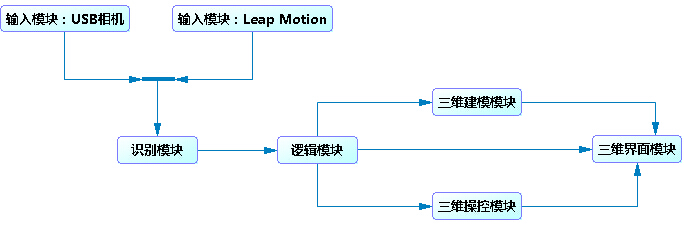
\includegraphics[width=0.8\textwidth]{chap2/system}
  \bicaption[fig:process]{系统概览图}{系统概览图}{Fig.}{system diagram}
\end{figure}

\section{系统介绍}
\subsection{系统概览}
本文系统着重研究混合现实眼镜下的交互界面、交互手段及空间设计应用中的具体设计,图\ref{fig:process}所示本文系统主要分为这几个模块:
输入模块、多通道识别模块、三维界面模块、逻辑模块、三维操控模块与建模模块。

%\begin{figure}[!htpb]
  %\centering
  %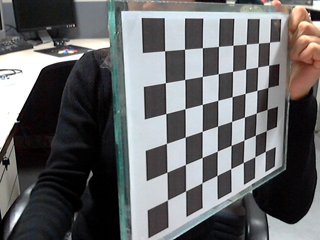
\includegraphics[width=0.24\textwidth]{chap2/camera_0_cap_1}
  %\hspace{1cm}
  %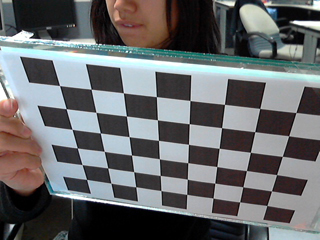
\includegraphics[width=0.24\textwidth]{chap2/camera_0_cap_2}
  %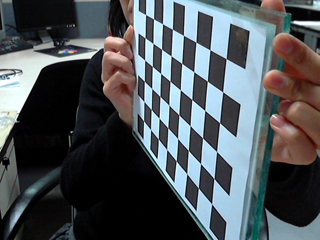
\includegraphics[width=0.24\textwidth]{chap2/camera_0_cap_12}
  %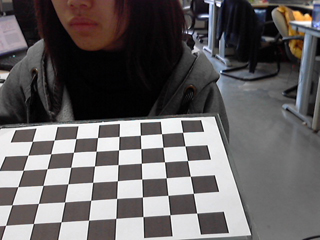
\includegraphics[width=0.24\textwidth]{chap2/camera_0_capture_1}
  %\bicaption[fig:chess]{棋盘格标定}{棋盘格标定}{Fig.}{Chessboard calibration}
%\end{figure}

\begin{figure}[!htpb]
	\centering
	\subfigure{\label{fig:chessboard:1}}\addtocounter{subfigure}{-2}
	\subfigure[Turn right]{\subfigure[向右偏转]
		{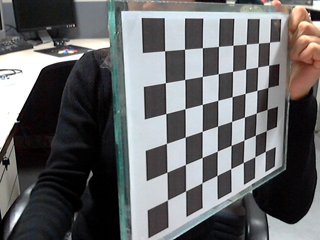
\includegraphics[width=0.22\textwidth]{chap2/camera_0_cap_1}}}		
	\subfigure{\label{fig:chessboard:2}}\addtocounter{subfigure}{-2}
	\subfigure[Turn down]{\subfigure[向下偏转]
		{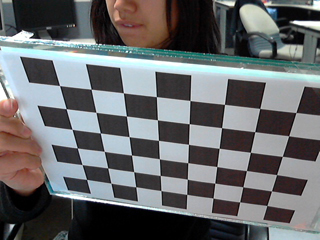
\includegraphics[width=0.22\textwidth]{chap2/camera_0_cap_2}}}		
	\subfigure{\label{fig:chessboard:3}}\addtocounter{subfigure}{-2}
	\subfigure[Turn left]{\subfigure[向左偏转]
		{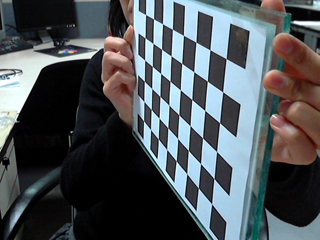
\includegraphics[width=0.22\textwidth]{chap2/camera_0_cap_12}}}	
	\subfigure{\label{fig:chessboard:4}}\addtocounter{subfigure}{-2}
	\subfigure[Turn up]{\subfigure[向上偏转]
		{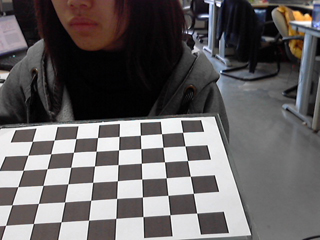
\includegraphics[width=0.22\textwidth]{chap2/camera_0_capture_1}}}		
	\bicaption[fig:chess]{棋盘格标定}{棋盘格标定}{Fig.}{Chessboard calibration}
	%\bicaption[总标签名]{}{中文总标题}{Fig.$\!$}{The total caption}
	\vspace{-1em}
\end{figure}

\subsection{输入与识别模块}
\label{sec:input}
	
本文系统在设计过程中涉及多种输入方式,本模块负责所有输入的标定。本文所设计的系统使用自制的混合现实眼镜ARGlasses作为系统输入,ARGlasses在演变过程中由不同硬件设备组成,输入部分有USB Camera, Leap Motion及改装过的广角USB Camera。 
为了模拟双目视觉的效果,系统之初采用两个横置USB Camera,
如图\ref{fig:chess}所示通过棋盘格进行独立标定,获得所需内参,图\ref{fig:chess}(a)、\ref{fig:chess}(b)、\ref{fig:chess}(c)和\ref{fig:chess}(d)分别是上下左右四个方向尽力偏转标定的演示,而后再进行双目标定。
图\ref{fig:stereoCalibration}显示通过双目标定后对原图像进行变换,变换前可从图\ref{fig:stereoCalibration}(a)中观察到左右二图的不匹配,而后左右眼图像(图\ref{fig:stereoCalibration}(c)})对齐效果更佳,可从背景的一些水平纹理中看到。
\begin{figure}[!htpb]
  \centering  
  \subfigure{\label{fig:stereoCalibration:before}}\addtocounter{subfigure}{-2}
	\subfigure[Left image before calibration]{\subfigure[标定前的左图]
		{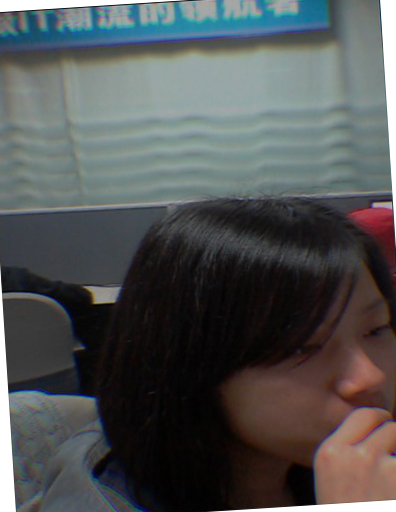
\includegraphics[width=0.225\textwidth]{chap2/beforeCalibration}}}		
	\subfigure{\label{fig:stereoCalibration:beforer}}\addtocounter{subfigure}{-2}
	\subfigure[Right image before calibration]{\subfigure[标定前的右图]
		{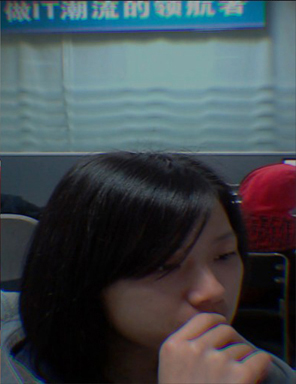
\includegraphics[width=0.225\textwidth]{chap2/afterCalibrationR}}}		
	\subfigure{\label{fig:chessboard:3}}\addtocounter{subfigure}{-2}
	\subfigure[Image after calibration]{\subfigure[标定后的图]
		{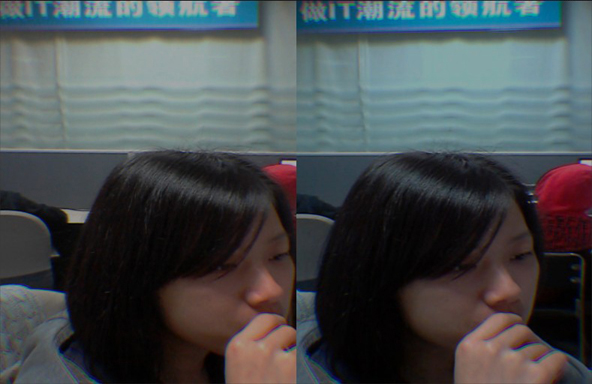
\includegraphics[width=0.45\textwidth]{chap2/afterCalibration}}}	
  \bicaption[fig:stereoCalibration]{双目标定}{双目标定}{Fig.}{stereo calibration}
\end{figure}
然后Leap Motion的采用是为了获得更稳定细致的手势信息,早期Leap Motion只提供具体的手部骨骼信息,为了将相机输入信息与Leap Motion的手部骨骼信息融合,系统自行设计了一套标定方法,系统通过在相同的位置呈现手势与棋盘格,获得多组对应数据进行点集映射得到粗略标定结果。
为了扩大捕捉到的场景视角,系统给相机增加了广角镜头,因此在输入处理过程中先对广角镜头捕获到的画面进行反扭曲处理,而后对反扭曲的结果进行棋盘格标定等操作,其效果可由图\ref{fig:WideLensUndist}可见。
棋盘格在图
\ref{fig:WideLensUndist}(a)中交叉线微微弯曲,而在图\ref{fig:WideLensUndist}(b)中反扭曲为直线,可见效果。

\begin{figure}[!htpb]
  \centering
  \subfigure{\label{fig:WideLensUndist:before}}\addtocounter{subfigure}{-2}
	\subfigure[Image before wide lens undistortion]{\subfigure[广角镜头反扭曲前的图]
		{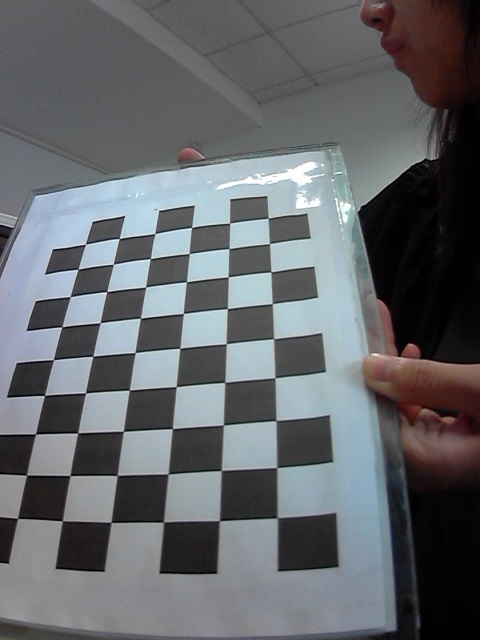
\includegraphics[width=0.3\textwidth]{chap2/camera_1_capture_6}}}		
	\subfigure{\label{fig:WideLensUndist:after}}\addtocounter{subfigure}{-2}
	\subfigure[Image after wide lens undistortion]{\subfigure[广角镜头反扭曲后的图]
		{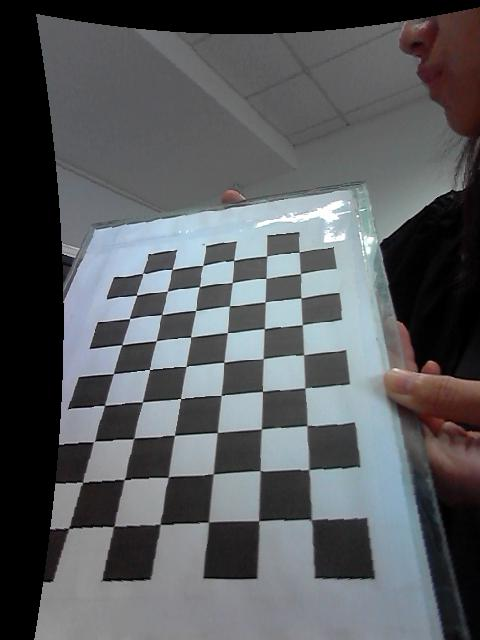
\includegraphics[width=0.3\textwidth]{chap2/undistcamera_1_capture_6}}}
  \bicaption[fig:WideLensUndist]{广角镜头反扭曲前后对比图}{广角镜头反扭曲前后对比图}{Fig.}{Undistortion of USB camera with wide lens}
\end{figure}

在研究的过程中,Leap Motion提供图像接口,可以获取拍摄所得源图像,于是系统结合Leap Motion所获取的源图像与相机图像进行匹配。
通过Leap Motion得到的原图进行反扭曲处理,由图\ref{fig:LeapMotionUndist}可见前后对比,棋盘格在图
\ref{fig:LeapMotionUndist}(a)中向右偏转,图\ref{fig:LeapMotionUndist}(b)中正面向前,图\ref{fig:LeapMotionUndist}(c)中向右偏转,然后将其作为混合现实眼镜的背景。
本模块最终输出标定过后的图像或手势信息,供识别模块进一步处理。
虽然输入模块相当重要,但并非本文重点所以之后并不再赘述。

\begin{figure}[!htpb]
  \centering
  \subfigure{\label{fig:LeapMotionUndist:left}}\addtocounter{subfigure}{-2}
	\subfigure[Turn right]{\subfigure[向右转]
		{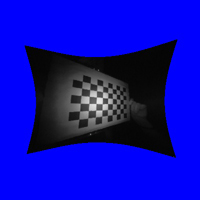
\includegraphics[width=0.3\textwidth]{chap2/undistort_399}}}		
	\subfigure{\label{fig:LeapMotionUndist:face}}\addtocounter{subfigure}{-2}
	\subfigure[Face to face]{\subfigure[正面]
		{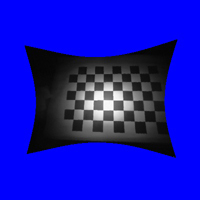
\includegraphics[width=0.3\textwidth]{chap2/undistort_299}}}		
	\subfigure{\label{fig:LeapMotionUndist:right}}\addtocounter{subfigure}{-2}
	\subfigure[Turn left]{\subfigure[向左转]
		{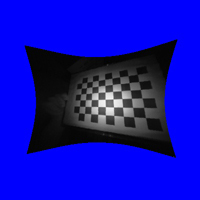
\includegraphics[width=0.3\textwidth]{chap2/undistort_219}}}
  \bicaption[fig:LeapMotionUndist]{Leap Motion反扭曲图}{Leap Motion反扭曲图}{Fig.}{Undistortion of Leap Motion images}
\end{figure}

识别模块主要有相机识别手势,Leap Motion识别手势,Oculus VR\upcite{Oculus}识别头部动作构成。
相机识别手势有以下几个步骤,首先获取原彩色图进行肤色提取,考虑到色彩空间在不同光线下并不稳定,所以这里设定了较广的肤色阈值,而后对超过手型大小阈值的肤色区域进行手型识别,根据形状判断是否含有手指,含有合法手指的区域便认定为是手型。标准的手型提取便是如此,之后根据手势的设计会有更细致的修改。
Leap Motion识别手势比较便捷,该设备官方提供手部骨架,可以直接分析其动作。
Oculus VR内置传感器,可以获得当前设备的角度,因而可以分析头部的动作信息,判断是否上仰。

\subsection{三维界面模块}
\label{sec:interface}
三维界面模块维护文所设计的系统界面,本文系统为混合现实眼镜设计了独有的三维界面,用来更好地配合用户的操作进行显示与交互。
三维界面由调色盘菜单和其他辅助信息组成,调色盘菜单地位等同桌面应用下的WIMP系列\upcite{Behr:2008:CND:1401132.1401164},负责让用户更直观地选择想要的命令。
其他辅助信息包括选中的立体包围盒,顶置提示板,骨骼小球都是本文所设计的系统运行中帮助用户更好地体验混合现实眼镜的可选配置,将在第\ref{chap:exp}章详细描述并评估。

\subsection{逻辑与操控模块}
\label{sec:logic}
逻辑模块负责连接识别结果与具体操作。结合识别到的手势,当前的环境,判断手势想表达的含义,比如在菜单出现时单手手指表示选择,而在物体被选中时表示单手操控。
据此调整三维界面上的显示,包括在顶置布告栏上更新状态,更改被选中的菜单样式进行提醒等。
逻辑模块还将输出具体指令下的操作参数,如旋转操作的轴参数与角度参数,传递给三维操控模块。

三维操控模块负责基本的平移旋转和缩放操控,通过输入的参数判断是哪种操控类型,然后根据参数进行实施操控,包括单手旋转和双手旋转时不一样的操控方式,也在该模块的处理之中。

\subsection{建模模块}
\label{sec:model}
建模模块针对三维建模用例,负责将用户的一系列建模指令转换成顶点。根据本文系统设计的自由虚拟网格平面,用户的输入全部转化为控制点,根据控制点该模块将绘制网格形成三维模型。
由于控制点的顺序随用户自定,所以该模块首先根据所有的控制点进行最优凸多面性估测用户绘制的形状,然后将不同层之间的控制点连接成三角面片。
除此之外在建模过程中自由虚拟网格平面的网格大小与方向都可由用户控制变换,针对被放缩与旋转的情况根据中心变换原则对所有控制点和网格平面进行点的相对位置的变换。在后文自由虚拟网格平面的具体设计中会详细描述。

\subsection{混合现实眼镜设备}
\label{chap:ARGlasses}

\subsubsection{混合现实眼镜初代}
\begin{figure}[!htp]
  \centering
  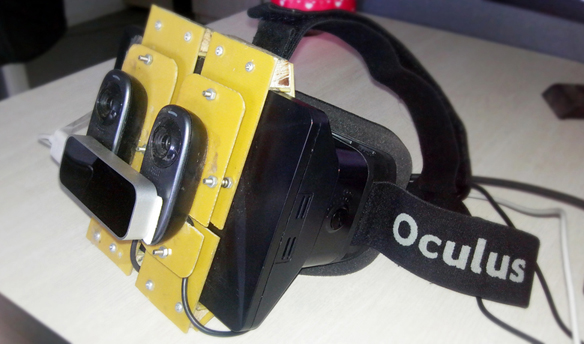
\includegraphics[width=0.6\textwidth]{chap2/ARGlassv1}
  \bicaption[fig:ARGlassesV1.0]{ARGlasses V1.0}{ARGlasses V1.0}{Fig.}{ARGlassesV1.0}
\end{figure}
图\ref{fig:ARGlassesV1.0}为混合现实眼镜的最初设计,由两个USB相机捕获彩色数据,放置在最前方,由Leap Motion捕获手指骨骼,安置在中间,然后通过自制的固定夹板将输入设备固定在Oculus VR上,用户可以通过Oculus VR看到输入设备捕获的现场从而达到视频透视。
在夹板上设有许多旋钮,可以简单调整相机的位置与角度,使两个相机互相间尽量保持一致的相对位置,且达到理想的标定误差。
初代设计的缺陷其一是质量太重,在实验过程中几乎所有参与者都在摘下眼镜后眼睛略感不适并反馈有点沉。
其二则是视野太窄,一个普通摄像头的水平视角在39°,垂直视角在31°,为了达到双目效果横置两个摄像头,于是每个眼睛的水平视角则为31°,与人眼本身接近平角的观察范围相差甚远,观察到的景象会有放大的感觉,让用户失去对深度的正确判断,故而第二个版本主要针对视角进行修改。

\subsubsection{混合现实眼镜广角版}
\begin{figure}[!htp]
  \centering
  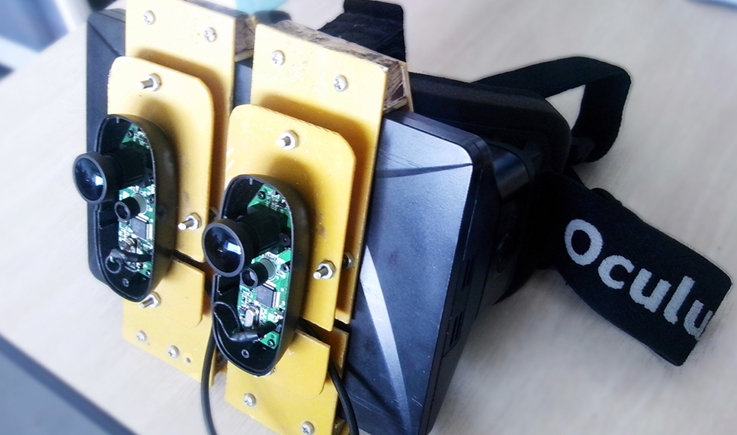
\includegraphics[width=0.6\textwidth]{chap2/ARGlassv2}
  \bicaption[fig:ARGlassesV2.0]{ARGlasses V2.0}{ARGlasses V2.0}{Fig.}{ARGlassesV2.0}
\end{figure}

图\ref{fig:ARGlassesV2.0}主要针对视角进行修改,可以看到原先的USB相机被拆到电路板层级并在摄像头元件前端安置了两个180°广角镜头,安装之后水平视角达到72°,虽然距离人眼的自然视角仍有距离,但比初代版本要宽广一些,并且质量上并没有很大变化。
但初代和广角版共同的缺陷在于双目相机之间的标定,双目标定可以做到对某一深度的物体进行匹配,从而左右眼可以合作观察该深度的物体,但是对于其他深度就会出现标定不合的情况,这是自制双目相机与视频透视融合的缺陷,也是接下来要解决的主要问题。

\begin{figure}[!htp]
  \centering
  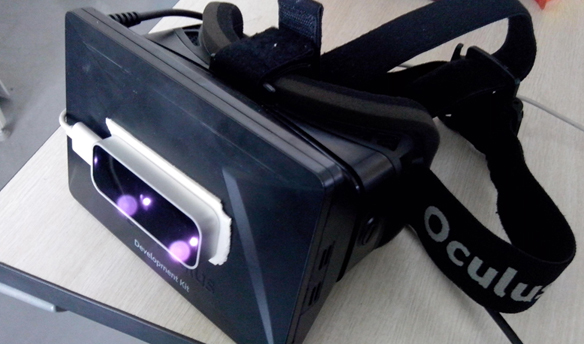
\includegraphics[width=0.6\textwidth]{chap2/ARGlassv3}
  \bicaption[fig:ARGlassesV3.0]{ARGlasses V3.0}{ARGlasses V3.0}{Fig.}{ARGlassesV3.0}
\end{figure}

\subsubsection{混合现实眼镜轻量级}

图\ref{fig:ARGlassesV3.0}则是最新版本,出于轻便性、视野及图像匹配的考虑,本文所设计的系统放弃彩色图像来源,直接使用Leap Motion作为唯一图像输入。
Leap Motion由于本身设备使用多角度的红外摄像头加灰阶Camera采集,可以捕捉到黑白景象,黑白灰阶随深度和热量而变。
其分辨率为640*240,虽然不高但和显示设备Oculus VR的800*600也相去不远。
\begin{table}[!hptb]\renewcommand{\arraystretch}{1.2}
  \centering
  \bicaption[table:arglass]{本文工作所制作的三代混合现实眼镜对比}{本文工作所制作的三代混合现实眼镜对比}{Table}{Comparison among three generations of Mixed Reality Glasses in this work}
  \begin{tabular}{*{4}{L{.32\textwidth}}} \toprule
  %\begin{tabular}{@{}ccc@{}} \toprule
    眼镜名称 & 优点 & 缺点 \\
	\midrule
    混合现实眼镜初代 	& 		1.彩色图像 		& 	\hspace{150pt}1.笨重\hspace{90pt}2.视野狭窄\hspace{90pt}3.存在设备间标定误差\\	
	%&&2.视野狭窄\\
	%&&3.存在设备间的标定误差\\
	%\vspace{1em}
    混合现实眼镜广角版 & 1.彩色图像\hspace{80pt}2.视野有扩大\vspace{1em}& 1.仍显笨重\hspace{90pt}2.存在设备间标定误差\\
	%&2.视野有扩大 &2.存在设备间的标定误差	\\
	%\vspace{1em}
    混合现实眼镜轻量级 & 1.视野符合人眼\hspace{100pt}2.轻巧\hspace{100pt}3.单一输入设备无标定误差& 1.灰色图像 \\
	%&2.轻巧 &\\
	%&3.单一输入设备无标定误差&\\
	\bottomrule
  \end{tabular}
\end{table}
关键其一他的视角到达110°以上,戴上之后和直接视物差距不大,其二由于是将一个完整的场景分割为左右眼两幅图像传递给用户,于是并没有两幅图像间不匹配的困扰,同时由于少了USB相机和固定用的夹板,整个设备一下子轻了很多。
最终三维界面与操控的设计基于混合现实眼镜初代,而三维建模应用的设计基于混合现实眼镜轻量级实现。

\section{本章小结}
本章概要地描述了本文系统的研究方法,然后介绍了本文系统的流程与模块划分,通过本章可以直观明朗地了解到本文系统的输入输出与用例,方便在对其中细节更深的探索前有一个完整的概念。
然后介绍了本文所设计的系统依赖的硬件设备:自制的混合现实眼镜,讲述其构造与发展历程,三代混合现实眼镜的比较可见表\ref{table:arglass}。
本文系统都构建在该设备之上,虽然硬件制作不是本文的重点,但其准确率、精度与轻便性对本文所设计的系统的实验评估都有很大影响,在此处特别介绍下。

%%==================================================
%% chapter03.tex for SJTU Master Thesis
%% Encoding: UTF-8
%%==================================================

\chapter{混合现实眼镜下的三维界面设计}
\label{chap:3DUI}

本章将介绍本文所设计的混合现实眼镜交互系统的第一个部分:三维界面。
三维界面的想法来源于增强现实应用中用户所触及到的三维事物。
大家已经熟悉的桌面应用界面为WIMP系列,二维的界面对应二维的输入,而现在手机、平板上的界面也开始随着设备慢慢地变化,由此本文所设计的系统根据整个操控环境都是三维的前提专门设计了一套三维界面。首先介绍适合增强现实交互界面的设计原则,接着呈现效果,这套三维交互界面将应用在第\ref{chap:interaction}章的交互研究中。

\section{设计原则}

基于\ref{sec:related-cur}节调研的研究现状,本节首先总结出适合增强现实交互界面的设计原则。
该原则主要为避免对识别准确性的影响,减少用户的记忆负担,同时增强交互的用户体验,列举如下:

\label{sec:design-principle}
\begin{enumerate}
\item 不在手上佩戴笨重的设备

由\ref{sec:related-jiaohu}节提到的相关工作可以看到不少精心制作的增强现实设备,然而若是佩戴复杂或者笨重的设备在手上会导致两个问题。
其一,用户体验下降,除了交互之外用户还会被设备的触感,重量等干扰,无法更自如地进行交互;
其二,用户极有可能在使用过程中对设备造成人为影响,比如无意中影响了预设的配置环境,旋转了uTrack\upcite{uTrack}
上的传感器,就会影响输入检测的正确性。
因此从舒适性和正确性角度出发,本文系统的设备将尽量减少手上复杂或笨重的设备佩戴。

\item 保持交互的一致性

试想如果一个增强现实应用中的操控和物理世界有着对应,却用着截然不同的交互手段,则势必会影响用
户在操控时的感受,并且增加记忆的复杂度。所以尽量保留物理世界的交互方式有助于用户尽快适应系统。
同时在物理世界无法做到的功能上,体现增强现实交互的优势,比如用户无法碰触远方的物体因而无法操控,但在增强现实应用环境下就可以实现这一点,
本文工作在对交互一致性的保持上进行改进的设计。

\item 尽可能少的手势设计

这一点同样是出于帮助用户快速适应改进后系统的考虑。
如果一个系统的手势指令太多,用户的记忆复杂度就会增加,可能需要进行一定时间的训练或者每次
都要仔细回顾一番才能再一次适应该系统。
为了让用户迅速学会使用该系统且经久不忘,本文系统最终只设计了三个手势,将在第\ref{chap:interaction}章中详述。

\item 明显的状态切换

在\ref{sec:related-zhuangtai}节中提到通过遮盖两个图案来进行状
态切换的系统\upcite{TrackingBased}。
在实验中,用户经常忘记遮盖指定图案来发送指令,也就是由于状态切换的指令不够明显和
简单,给使用者增加了难度,导致用户的错误指令,
故而系统将设计简单明了的状态切换方式,提升易用性。

\end{enumerate}

根据以上原则,本文设计了手掌召唤式菜单、目标跟踪式菜单和屏幕固定式这三种菜单,具体阐述如下。

%\section{设计结果展示}

\section{手掌召唤式菜单}
\label{sec:palm-based}
\begin{figure}[!htp]
  \centering
  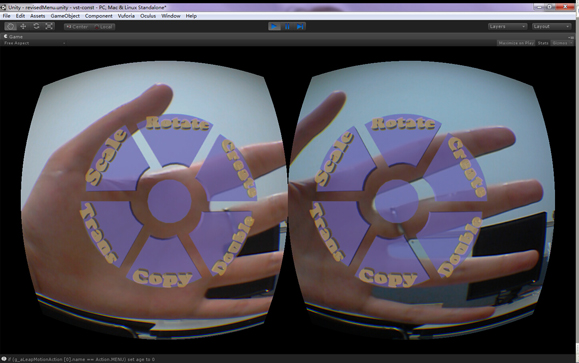
\includegraphics[width=0.8\textwidth]{chap3/palm-basedMenu}
  \bicaption[fig:palm-based]{手掌召唤式菜单}{手掌召唤式菜单}{Fig.}{Palm-based menus}
\end{figure}

手掌召唤式菜单是用户通过手掌手势召唤而
成的菜单,顾名思义位置始终固定在手掌上。为了让菜单和用户
更加融合,本文所设计的系统依据手掌的形状,借鉴调色盘的
概念设计出了该菜单,也是区别于以往直接将二维菜单或者基本图元照搬的一个特点。
用户通过拣选菜单上不同的
指令,然后选中物体对其进行相应的操作,就如同
将调色盘上不同的颜色分配在不同的物体上一样。
如图\ref{fig:palm-based}所示,当摄像头捕获到菜单指令后,在用户手掌正中心出现的就是该菜单,就像是用户手握的一个道具一样。

手掌召唤式菜单含有以下几个选项:创建物体、单手移动物体、单手旋转物体、单手放缩物体、双手操控物体和拷贝物体。
操控类菜单选中后需要指定目标物,可以一个,可以多个。
用户单手操控物体时需要选择不同指令进行不同操作,而用户双手操控物体时,只需要选择双手操控物体的命令即可。
随后系统将根据用户双手间的相对移动,以时间为轴判断用户在进行平移放缩还是旋转。

\section{目标跟踪式菜单}
\begin{figure}[!htp]
  \centering
  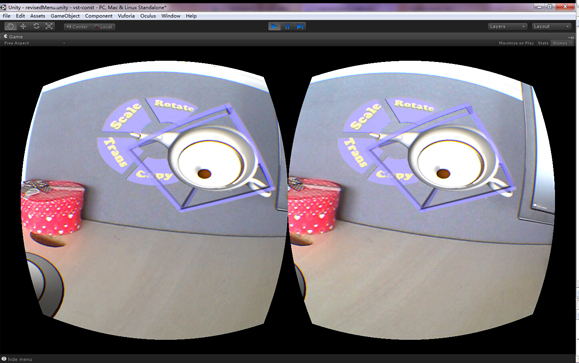
\includegraphics[width=0.8\textwidth]{chap3/object-trackedMenu}
  \bicaption[fig:object-tracked]{目标跟踪式菜单}{目标跟踪式菜单}{Fig.}{object-tracked menus}
\end{figure}

目标跟踪式和手掌召唤式菜单触发方式属于两种类型,后者通过用户的手召唤出来,是基于操作的一种菜单调用;
而前者则是通过选中场景内已经存在的物体,目标跟踪式菜单会出现在该物体周围,随物体的位置变化而变化,选择具体的指令后,该指令就会作用在被选中的物体上,属于基于目标物的一种菜单调用。
如图\ref{fig:object-tracked}所示,召唤出的菜单卡在被选中目标物的一侧。

目标跟踪式菜单有以下几个选项:单手移动物体,单手旋转物体,单手放缩物体,双手操控物体和拷贝物体。和\ref{sec:palm-based}节的功能描述类似。
在操作顺序上由于已经选中物体,于是选完菜单后就可以直接进行操控。

\section{屏幕固定式菜单}
\begin{figure}[!htp]
  \centering
  \subfigure{\label{fig:screen-fixed:1}}\addtocounter{subfigure}{-2}
	\subfigure[Screen-fixed menus sample one]{\subfigure[屏幕固定式菜单示例一]
		{\includegraphics[width=0.4\textwidth]{chap3/screen-fixedMenu1}}}
	\subfigure{\label{fig:screen-fixed:2}}\addtocounter{subfigure}{-2}
	\subfigure[Screen-fixed menus sample two]{\subfigure[屏幕固定式菜单示例二]
		{\includegraphics[width=0.4\textwidth]{chap3/screen-fixedMenu2}}}
  \bicaption[fig:screen-fixed]{屏幕固定式菜单}{屏幕固定式菜单}{Fig.}{Screen-fixed menus}
\end{figure}

屏幕固定式菜单和目标跟踪式菜单的触发方式相同,都属于基于目标物的菜单调用,但选中物体后,屏幕固定式菜单会固定在屏幕正中央,无论选中的物体在哪里,用户如何改变视角,该菜单都会出现在相同的位置,大小和角度都不会变化。
如图\ref{fig:screen-fixed}(a)所示,当选中了茶壶后,茶壶附近出现选中立体框,并在屏幕正中央出现菜单,
而后佩戴ARGlasses的用户向左转头如图\ref{fig:screen-fixed}(b)所示,整个场景变动,茶壶不在视野范围内,但该菜单依然固定在屏幕正中央。

以上三种菜单中,手掌召唤式菜单属于基于操作的菜单类型,选择统一的菜单指令后,可以将指令附着到多个物体上。
而目标跟踪式菜单与屏幕固定式菜单从单个物体出发,偏向个性化操作。
三种菜单在混合现实眼镜下的效果会在第\ref{chap:exp}章详细评估。

\section{三种布局的菜单对照与分析}

\begin{table}[!hpbt]\renewcommand{\arraystretch}{1.1}
  \centering
  \bicaption[table:3dmenu]{本文工作所设计的三种菜单对比}{本文工作所设计的三种菜单对比}{Table}{Comparison among three styles of 3D menus in this work}
\begin{tabular}{*{4}{L{.23\textwidth}}} \toprule
    分析内容 & 手掌召唤式菜单 & 目标跟踪式菜单 & 屏幕固定式菜单 \\
	\midrule
    特点描述 	&
	随手掌召唤而出,位置随手变化 		&
 	由选中物体触发,位置随物体变化 &
	%\vspace{1em}
	\hspace{100pt}由选中物体触发,位置固定在屏幕正中央\\	
	%\vspace{0.5em}
	设计原则一:\hspace{15pt}不在手上佩戴笨重的设备 &
	无任何佩戴物 &
	需佩戴色环选中物体 &
	需佩戴色环选中物体 &\\
%	\vspace{0.8em}
	设计原则二:\hspace{15pt}保持交互的一致性 &
	额外设计手掌触发菜单 &
	选中物体出菜单,与二维菜单习惯一致 &
	选中物体出菜单,与二维菜单习惯一致 &\\
%	\vspace{1em}
	设计原则三:\hspace{15pt}尽可能少的手势设计&
	新增手掌手势&
	选择手势与日常选中手势相似&
	选择手势与日常选中手势相似&\\
%	\vspace{0.3em}
	设计原则四:\hspace{15pt}明显的状态切换&
	通过手掌识别菜单模式&
	通过色环分离控制与选择指令&
	通过色环分离控制与选择指令&
	\bottomrule
  \end{tabular}
\end{table}

由表\ref{table:3dmenu}可见本文设计的三种布局的菜单。手掌召唤式菜单随手掌召唤而出,然后指定物体,是操作先于目标的一种思考方式,
目标跟踪式菜单指定物体然后显示,和屏幕固定式菜单相同,是目标先于操作的一种思考方式。
而这二者的区别在于菜单的位置,前者随目标物移动,而后者固定在屏幕中央。
前者的设计思路将菜单作为目标物的一种属性,将菜单镶嵌在目标物周围;
后者从更直观的显示角度出发。
在设计原则的应用上,三者都尽量减少了额外的佩戴物,即便是色环也是轻量级的物体;
手掌召唤式菜单额外增加了手掌召唤菜单的交互,但并没有和现实生活中的交互产生矛盾,对用户产生的记忆压力也不大,另两者没有新增交互和手势设计;
最后手掌手势和色环成功分离了自己的状态和其他状态,做到了明显的状态切换这一原则。

\section{本章小结}
本章主要介绍了本文所设计的系统使用的三维界面。
首先通过对相关工作的理解提出了设计原则,设计原则应用于三维界面设计。
然后列举了设计的三种菜单。
手掌召唤式菜单以操作为重点,先选菜单再选目标物,并且手掌召唤式菜单卡位于掌心,将用户的手变成了一个增强现实界面。
目标跟踪式菜单和屏幕固定式菜单均以目标物为重点,先选择想要操作的物体,然后再选择想要实行的功能。
并且采用了两种风格的布局,目标跟踪式菜单会随目标物而移动,屏幕固定式菜单则始终固定在屏幕正中央,无论用户看向何方都能看到嵌在屏幕中央的菜单,便于选择。
除此之外介绍了本文系统设计的几个菜单,分别是创建、单手操控菜单组、双手操控和拷贝物体。
对菜单进一步的评估将在第\ref{chap:exp}章展开。
%%==================================================
%% chapter03.tex for SJTU Master Thesis
%% Encoding: UTF-8
%%==================================================

\chapter{混合现实眼镜下的空间交互设计}
\label{chap:interaction}

本章结合上一章设计的三维界面,设计本文系统的第二个部分:空间交互。
本文系统采用以手势交互为主结合其他辅助方式的交互方法。
先介绍本文系统所使用的三个手势的设计思想与实现细节,
然后本文系统根据第\ref{chap:exp}章阐述的可行性实验评估结果优化,设计了多项辅助方式,分别是顶置提示板、骨骼小球和头部约束帮助用户进行空间交互。



\section{三维界面上的手势设计与实现}
%\begin{figure}[!htp]
  %\centering
  %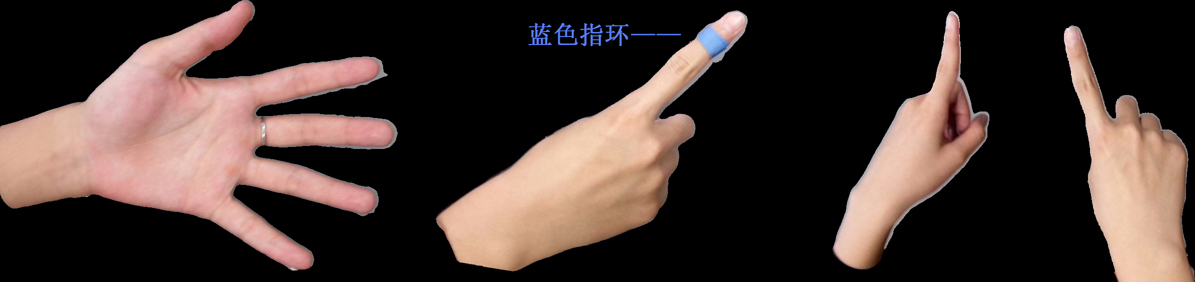
\includegraphics[width=0.6\textwidth]{chap4/gesture}
  %\bicaption[fig:gestures]{三种手势}{三种手势}{Fig.}{Three gestures}
%\end{figure}

\begin{figure}[!htp]
	\centering
	\subfigure{\label{fig:gestures:menu}}\addtocounter{subfigure}{-2}
	\subfigure[Menu gesture]{\subfigure[菜单手势]
		{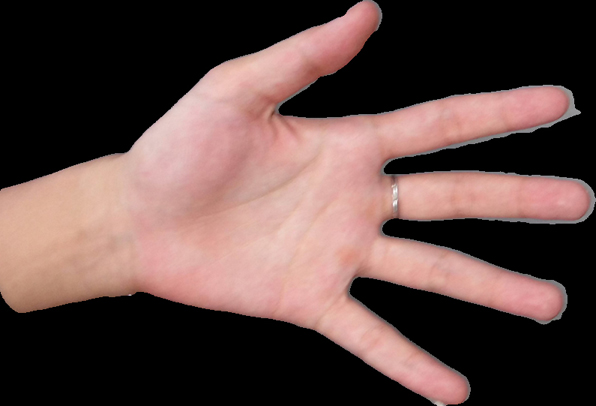
\includegraphics[width=0.32\textwidth]{chap4/gesture-menu}}}
	\subfigure{\label{fig:gestureselect}}\addtocounter{subfigure}{-2}
	\subfigure[Selection gesture]{\subfigure[选择手势]
		{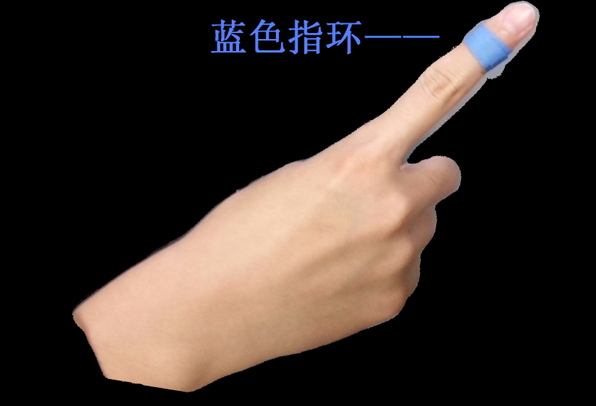
\includegraphics[width=0.32\textwidth]{chap4/gesture-select}}}
		\subfigure{\label{fig:gesture:manipulate}}\addtocounter{subfigure}{-2}
	\subfigure[Manipulation gesture]{\subfigure[操控手势]
		{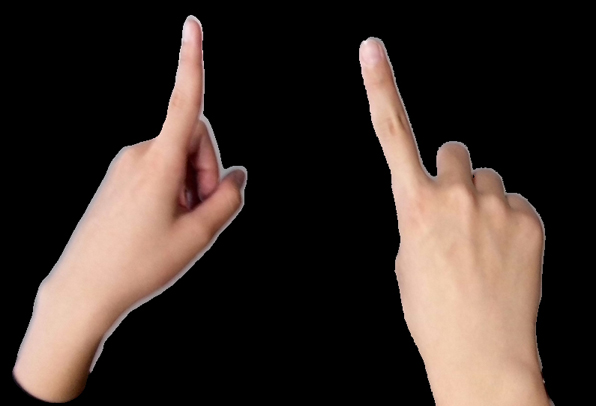
\includegraphics[width=0.32\textwidth]{chap4/gesture-mani}}}
	\bicaption[fig:gestures]{三种手势}{三种手势}{Fig.}{Three gestures}
	%\bicaption[总标签名]{}{中文总标题}{Fig.$\!$}{The total caption}
	\vspace{-1em}
\end{figure}

由\ref{sec:design-principle}节提到的设计原则,本文系统一共设计了三个手势:菜单手势、选择手势和操控手势。
由图\ref{fig:gestures}(a)可见,菜单手势即五指自然张开,本文系统检测到时便会将手掌召唤式菜单安置在掌心位置。
由图\ref{fig:gestures}(b)所示,选择手势使用色环触发,另一只手的手指戴上一个蓝色色环后,本文系统进入选择模式,如图\ref{fig:logicRelationship}所示,此刻无论是召唤菜单或者操控物体都不能进行,只能进行对菜单或者物体的选择。
当手指悬停选中菜单一定时间后,菜单消失表示指令已被选中。
根据所选的菜单选项,使用单手或双手进行操控,每只手自然伸出一根手指如图\ref{fig:gestures}(c)所示,即可对当前被选中的物体们进行操控。

本文中提到的操控是物体的几种基本操控:平移,旋转和缩放。

\begin{figure}[!htp]
  \centering
  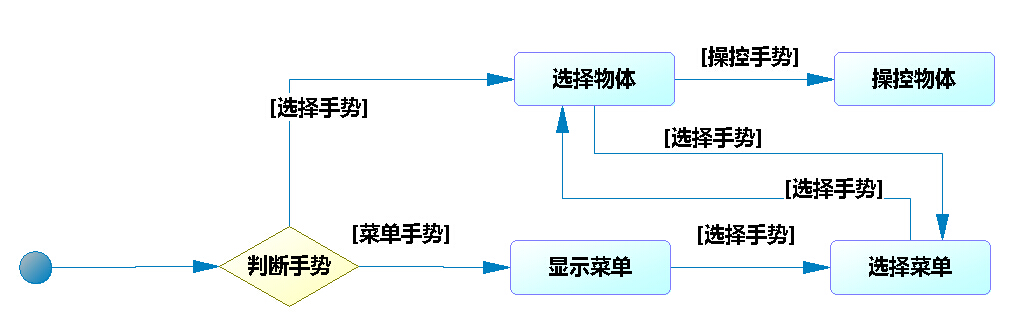
\includegraphics[width=0.95\textwidth]{chap4/gestureLogic}
  \bicaption[fig:logicRelationship]{三种手势的逻辑关系图}{三种手势的逻辑关系图}{Fig.}{the logic relationship among three gestures}
\end{figure}

\subsection{菜单手势}

菜单手势针对手掌召唤式菜单所设计,由USB相机输入的图像和Leap Motion输入的图像结合分析。
通过手指检测算法先判断USB相机的输入图像中是否有肤色区域内含五根手指,为了增加容错率,本文系统后期改为检测至少四根手指。
另一方面从Leap Motion处获得手部骨架,两处输入同时判断:是否同为左手或右手,如果不是,本文系统将当前手势信息状态置空;自然伸出的手指数量是否一致,
如果数量不一致则不继续;在两个输入一致通过检测后,本文系统利用先前粗略进行的Leap Motion和相机标定结果在手掌对应的位置绘制出调色盘菜单。
由于相机输入受环境影响颇大,此处对相机丢失信号的容忍度设了一个阈值T,只要在连续T帧内重新识别到手势,本文系统就继续显示调色盘菜单,反之则消失。

菜单手势实现算法如算法\ref{alg:menu}所示,先进行左右眼图像的立体匹配而后获取肤色区域,然后通过开操作和闭操作的降噪后获取最大的轮廓来进行判断是否有手指的存在。
	\begin{algorithm}  
		\caption{菜单手势实现算法}  
		\label{alg:menu} 
		\begin{algorithmic}  
		\REQUIRE{左右眼的两幅输入图像$Image_l_e_f_t$和$Image_r_i_g_h_t$}
		\ENSURE{手势类型$GestureType$和手指数据$HandInfo$}
			\STATE {对$Image_l_e_f_t$和$Image_r_i_g_h_t$进行立体匹配,校正图像}
			%\STATE {对左右眼的两幅输入图像进行色环提取}
			\STATE {对$Image_l_e_f_t$和$Image_r_i_g_h_t$进行肤色区域提取,为$Skin_l_e_f_t$和$Skin_r_i_g_h_t$}
			\FOR{each $image \in [Skin_l_e_f_t,Skin_r_i_g_h_t]$}
				\STATE {对$image$进行开闭等形态学降噪,为$image_i_m_p$}
				\STATE {获取$image_i_m_p$最大的两个轮廓$Hole_f$和$hole_s$}
				\FOR{each $hole \in [Hole_f,hole_s]$}
					\STATE {对$hole$多边形拟合进行手指识别,设置手指数据,手指数量记为$n$}
				\ENDFOR
				\IF{$n >= 4$}
					\STATE {$GestureType=MENU$}
					\STATE{填充$HandInfo$}
				\ENDIF
			\ENDFOR			
		\end{algorithmic}  
	\end{algorithm} 
\subsection{选择手势}

%\begin{description}
%\item[选择手势设计思想]\hfill\\
选择手势采用最常用的单手食指动作,模拟鼠标的左键,通常也是最常见的点击与选中意义。
然而如\ref{sec:input}节所提Leap Motion与相机间的粗略标定,当精确到需要提取用户指尖位置的时候,误差偏大因而这里采用了色环作为辅助工具。
色环颜色采用与肤色呈反色的蓝色调,简单易制作且轻量级几乎对用户没有任何压力。
同时自然地分割了移动与选中的状态切换。
当用户想要选中物体时,需佩戴上色环,此时摄像头捕捉到色环便默认用户正在进行选择,选择菜单或者选择目标物。
当摄像头没有捕捉到色环时,则对用户的手指移动进行操控手势的理解。

%\item[选择手势实现算法]\hfill\\
算法\ref{alg:select}详述了选择手势算法的实现。
其一考虑容错率,因而在转换成HSV空间的图像中对蓝色掉提取时放宽约束,捕获到场景内所有接近蓝色调的物体。
然后进行形态学闭操作,并根据区域大小大小过滤掉不符合要求的蓝色区域。
接着遍历所有候选者,与同时期获得的肤色区域进行闭操作。此时由于蓝色指环导致食指的肤色区域被分为两个部分,如果该候选者即色环区域,则这三个区域可以合并成为一根手指。
以关操作后是否成为一个连通域作为判断标准来寻找色环,增加了其稳定性。
而色环的位置也就是之后用户表示选中的位置。
由图\ref{fig:colorRing}可观察选择手势识别中的每一步的处理过程与结果展示

\begin{figure}[!htp]
	\centering
	\subfigure{\label{fig:colorRing:a}}\addtocounter{subfigure}{-2}
	\subfigure[Input image]{\subfigure[输入图像]
		{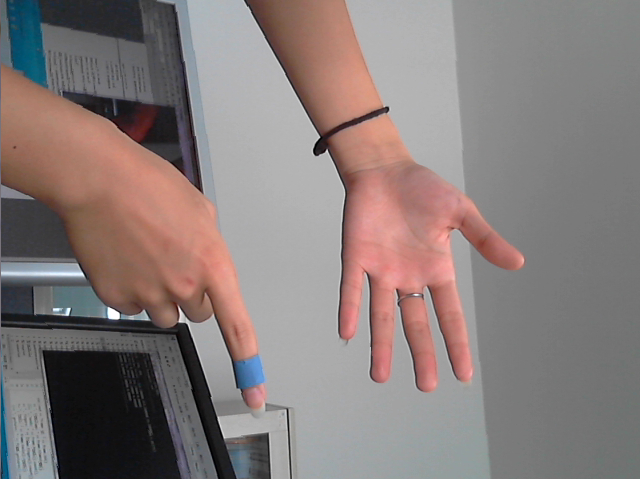
\includegraphics[width=0.3\textwidth]{chap4/color1}}}
	\subfigure{\label{fig:colorRing:b}}\addtocounter{subfigure}{-2}
	\subfigure[HSV color space]{\subfigure[HSV色彩空间]
		{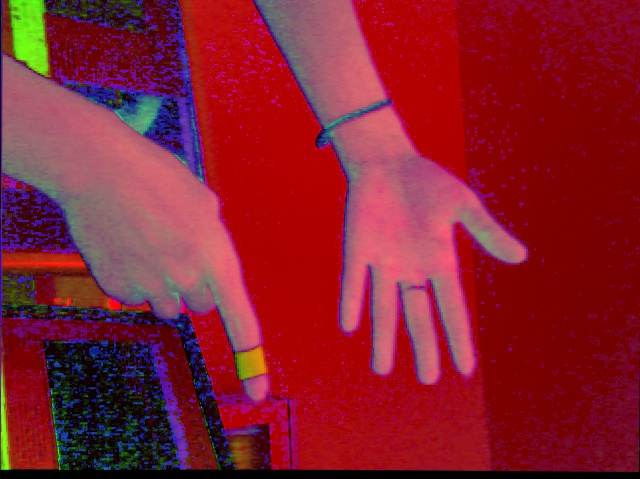
\includegraphics[width=0.3\textwidth]{chap4/color2-hsv}}}
	\subfigure{\label{fig:colorRing:c}}\addtocounter{subfigure}{-2}
	\subfigure[Skin extraction]{\subfigure[肤色提取]
		{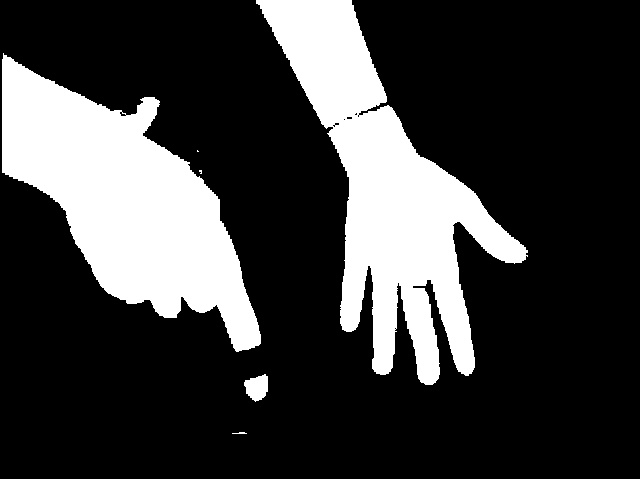
\includegraphics[width=0.3\textwidth]{chap4/color3-skin}}}
	\vspace{-1em}
	\subfigure{\label{fig:colorRing:menu}}\addtocounter{subfigure}{-2}
	\subfigure[Color ring extraction]{\subfigure[色环提取]
		{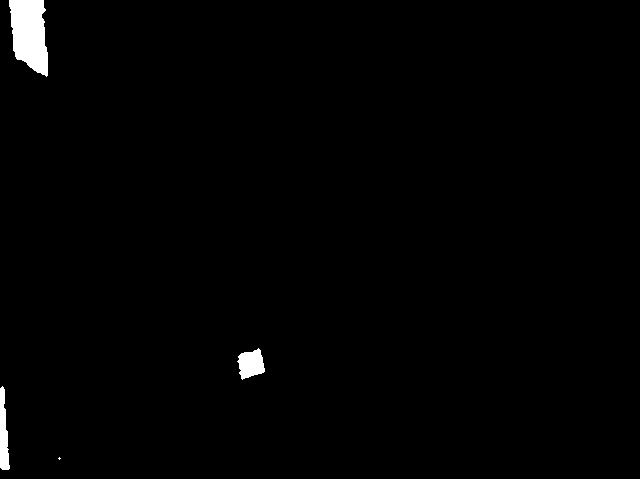
\includegraphics[width=0.3\textwidth]{chap4/color4-blue}}}
	\subfigure{\label{fig:colorRing:e}}\addtocounter{subfigure}{-2}
	\subfigure[Close operation]{\subfigure[闭操作]
		{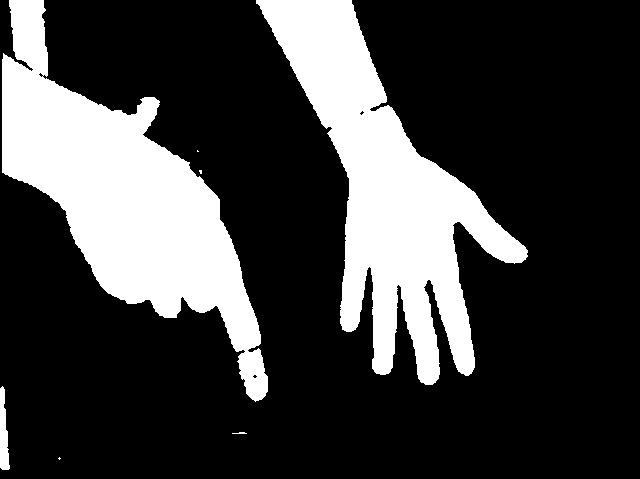
\includegraphics[width=0.3\textwidth]{chap4/color5-close}}}
	\subfigure{\label{fig:colorRing:f}}\addtocounter{subfigure}{-2}
	\subfigure[Mark color ring]{\subfigure[标记色环]
		{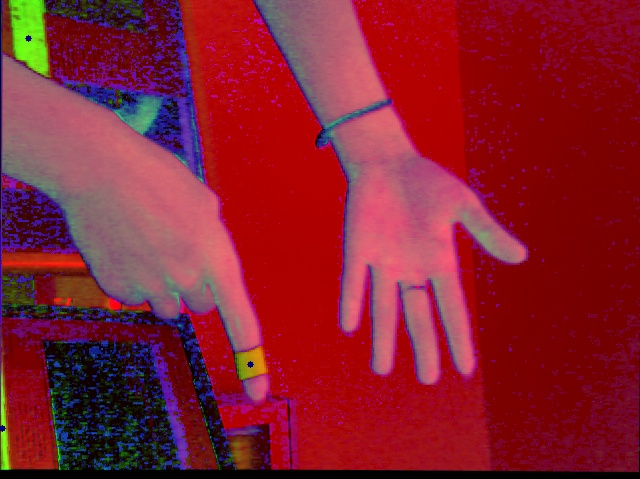
\includegraphics[width=0.3\textwidth]{chap4/color6-circle}}}
	\bicaption[fig:colorRing]{色环的处理过程}{色环的处理过程}{Fig.}{Process for color ring}
	%\bicaption[总标签名]{}{中文总标题}{Fig.$\!$}{The total caption}
	\vspace{-1em}
\end{figure}
	\begin{algorithm}  
		\caption{选择手势实现算法}  
		\label{alg:select} 
		\begin{algorithmic}
\REQUIRE{左右眼的两幅输入图像$Image_l_e_f_t$和$Image_r_i_g_h_t$}
\ENSURE{手势类型$GestureType$和手指数据$HandInfo$}
			\STATE {对$Image_l_e_f_t$和$Image_r_i_g_h_t$进行立体匹配,校正图像}
			\STATE {对$Image_l_e_f_t$和$Image_r_i_g_h_t$进行色环提取,记录$n$个候选色环点$circle_c_a_n_d$}
			\FOR{each $circle \in circle_c_a_n_d$}
				\IF{检测到色环}
					\STATE {对$Image_l_e_f_t$和$Image_r_i_g_h_t$进行肤色区域提取,为$Skin_l_e_f_t$和$Skin_r_i_g_h_t$}
					\FOR{each $skin \in [Skin_l_e_f_t,Skin_r_i_g_h_t]$}
						\STATE {对$skin$采用形态学开闭操作进行降噪,为$skin_i_m_p$}
						\STATE {获取$skin_i_m_p$最大的两个轮廓,为$contour_f$和$contour_s$}
						\FOR{each $contour \in [contour_f,contour_s]$}
							\STATE {将$contour$与色环候选区域合并}
							\STATE {形态学处理得到最大的轮廓$contour_m_a_x$}
							\FOR{each $i \in [1,n]$}
								\IF{判断候选点是否在轮廓范围内}
									\STATE{$GestureType=SELECT$}
									\STATE{填充$HandInfo$}
								\ENDIF
							\ENDFOR
							\STATE{如果均无则$GestureType=NULL$}
						\ENDFOR
					\ENDFOR	
				\ENDFOR
			\ELSE
				\STATE {$GestureType=NULL$}
			\ENDIF
		\end{algorithmic}  
	\end{algorithm} 

%\end{description}

%\begin{figure}[!htp]
  %\centering
  %\includegraphics[width=0.6\textwidth]{chap4/testpng}
  %\bicaption[fig:colorRing]{色环的处理过程}{色环的处理过程}{Fig.}{process for color ring}
%\end{figure}

\subsection{操控手势}

%\begin{description}
%\item[操控手势设计思想]\hfill\\
%\subsubsection{操控手势设计思想}
操控手势的设计思想在于操控手势不论单手双手都是用户自然伸直食指进行操控的。
区别在于具体的操控逻辑。
%\item[单手操控实现算法]\hfill\\
\subsubsection{单手操控实现算法}

单手操控时,首先选择具体指令。
如果是平移:平移的位移与手的位移一致,基本上就是直接对应的操作;
如果是旋转:旋转角度由手的移动距离决定,移动的距离越大则转的角度越多,而旋转轴由手的移动轨迹决定,基本和触摸屏操控一致,只不过没有固定触摸屏的限制于是用户可以进行譬如Z轴方向的移动;
如果是缩放,则根据常识向右向上向前为放大,反之为缩小,而缩放的幅度由手的位移决定。
%\item[双手操控实现算法]\hfill\\
\subsubsection{双手操控实现算法}

\begin{algorithm}  
		\caption{双手操控实现算法}  
		\label{alg:double} 
		\begin{algorithmic}  
		\REQUIRE{左右双手$Hand_l_e_f_t$和$Hand_r_i_g_h_t$,手的类型$HandType$,操控之手数量$m$,左右双手位置$pos_l_e_f_t$和$pos_r_i_g_h_t$,左右双手上一帧的位置$posPre_l_e_f_t$和$posPre_r_i_g_h_t$}
		\ENSURE{变换类型$TransType$和参数数组$para$}
		\STATE {$m=0$}
		\FOR{each $hand \in [Hand_l_e_f_t,Hand_r_i_g_h_t]$}
			\FOR{each $fingerIdx \in [1,5]$}
				\IF {手指自然伸直}
					\STATE {手指数量$n=n+1$}
				\ENDIF
			\ENDFOR
			\IF{$n == 1$}
				\STATE{$hand.HandType = MNPL$}
				\STATE {$m=m+1$}
			\ENDIF
		\ENDFOR
		\IF{$m == 2$}
			\STATE{$vec_c_u_r = pos_l_e_f_t-pos_r_i_g_h_t$}
			\STATE{$vec_p_r_e = posPre_l_e_f_t-posPre_r_i_g_h_t$}
			\STATE{$vec_l_e_f_t = pos_l_e_f_t-posPre_l_e_f_t$}
			\STATE{$vec_r_i_g_h_t = pos_r_i_g_h_t-posPre_r_i_g_h_t$}
			\STATE{$rotateAngle = angle(vec_c_u_r,vec_p_r_e)$}
			\IF{$rotateAngle <= \pi/9$}
				\STATE{$TransType = TRANS$}
				\STATE{$para[0] = (vec_l_e_f_t + vec_r_i_g_h_t) / 2$}
			\ELSIF{$rotateAgle >= \pi*5/6$}
				\STATE{$TransType = SCALE$}
				\STATE{$para[0] = vec_c_u_r / vec_p_r_e$}
			\ELSIF{$rotateAngle \in [\pi/6,\pi/2]$}
				\STATE{$TransType = ROTATE$}
				\STATE{$para[0] = cross(vec_l_e_f_t,vec_r_i_g_h_t)$}
				\STATE{$para[1] = rotateAngle$}
			\ENDIF
		\ENDIF
	\end{algorithmic}  
\end{algorithm} 
	
双手操控时,本文系统会同时判断是否在进行平移、旋转,和缩放,用户可以同时进行这些操控,具体算法见算法\ref{alg:double}。
本文系统对两只手的位移进行分析,分离两只手在X轴、Y轴和Z轴三轴上的矢量,如果在同一轴上的矢量是同向的,则取其均值作为平移参数,将符合条件的矢量相加得到最后的平移指令;
如果分离出是相向运动,则进行放缩,放缩的参数由该方向的移动后距离与移动前距离做比值,以该比值为参数调整目标物体的大小;
然后对左手和右手的移动路径做叉乘,看是否存在扭矩。
存在则以叉乘结果矢量为旋转轴,结果绝对值为旋转角度参数。
双手操控由于可以同时进行三种基本变换,因而省略了切换命令的步骤,并且同时发出多个指令也是的操控更为高效。
%\end{description}

\section{三维界面上的辅助设计}

在易用性用户实验后,根据用户的反馈与提议,本文所设计的系统增加了其他的辅助功能帮助用户更好地体验这一套三维菜单和三维操控手势。
以下为新增的辅助设计。

\subsection{顶置提示板}
\label{fig:interaction:board}
%\begin{figure}[!htp]
  %\centering
  %\includegraphics[width=0.3\textwidth]{chap4/testpng}
  %\hspace{1cm}
  %\includegraphics[width=0.3\textwidth]{chap4/testpng}
  %\bicaption[fig:board]{顶置提示板}{顶置提示板}{Fig.}{Board}
%\end{figure}
根据实验反馈,我们得到使当前系统状态更明朗化的提议,于是在用户视野的正上方显示了一个提示板,提示当前用户正在进行的操作,安置在正上方是为了让提示板的存在不影响到整体布局。
随着用户的操作,提示板的内容会因之变化,关于其布局位置与是否有存在价值将会在之后的实验具体说明。

\subsection{骨骼小球}
\label{sec:interaction:skeleton}
%\begin{figure}[!htp]
  %\centering
  %\includegraphics[width=0.4\textwidth]{chap4/skeletonball1}
  %\hspace{1cm}
  %\includegraphics[width=0.4\textwidth]{chap4/skeletonball2}
  %\bicaption[fig:skeletonball]{骨骼小球}{骨骼小球}{Fig.}{skeletonball}
%\end{figure}

另一修改点是关于Leap Motion。对不少实验者而言,Leap Motion也是一个全新的设备,并没有任何使用过的经验,于是实验中除了新增熟悉Leap Motion的步骤外,对于其在实验进行中的可视化也是一个辅助用户操作的办法。
这里的设计是增加了骨骼小球,而骨骼小球的位置与用户的手一一对应,用户可以通过观察骨骼小球的位置得知目前自己的手在Leap Motion系统中是什么情况,以及是否被正确识别。
因为最初的实验中经常遇到本文系统未对用户的操控进行响应的情况,而其原因大部分是Leap Motion并未捕捉到用户的手。
虽然Leap Motion和人眼的物理位置非常接近,但其视角的不同导致用户所见的场景并不是Leap Motion所见,于是骨骼小球的存在就可以用于提示用户。

\begin{figure}[!htp]
	\centering
	\subfigure{\label{fig:skeletonball:a}}\addtocounter{subfigure}{-2}
	\subfigure[Selection gesture with skeleton ball]{\subfigure[选择手势下的骨骼小球]
		{\includegraphics[width=0.4\textwidth]{chap4/skeletonball1}}}
	\subfigure{\label{fig:skeletonball:b}}\addtocounter{subfigure}{-2}
	\subfigure[Menu gesture with selection gesture]{\subfigure[菜单手势下的骨骼小球]
		{\includegraphics[width=0.4\textwidth]{chap4/skeletonball2}}}
	\bicaption[fig:skeletonball]{骨骼小球}{骨骼小球}{Fig.}{Skeleton ball}
	%\bicaption[总标签名]{}{中文总标题}{Fig.$\!$}{The total caption}
	\vspace{-1em}
\end{figure}

如图\ref{fig:skeletonball}所示,相同颜色的骨骼小球表示相同的手指,如果视野中未出现一个骨骼小球,表示当前检测不到任何有效的手。
通过观察骨骼小球,用户可以调整自己的手势来更好地操控。
对于骨骼小球布局及存在价值,会在进一步的实验中详细验证。

\subsection{头部约束}
\label{sec:interaction:head}
头部约束的想法来源与手掌召唤式菜单,手掌召唤式菜单的动作与其说是显示自己的手心,更接近一个翻转手腕的动作,而这个动作通常以低头完成更加自然。
于是针对部分用户反馈的菜单过于容易被触发的问题,改进后的系统中增加了对手掌召唤式菜单的头部约束,模拟画家画画时的景象,选用调色盘上的颜
料时,总是低头看向捧着的调色盘。于是改进后的系统中约束用户只有在低头的时候才能触发该菜单,一方面避免了菜单无意中被触发的情况,另一方面帮助
用户将菜单操作区域和虚拟物体操作区域划分得更清楚,减少无意中选中物体的情况。

\begin{figure}[!hpb]
	\centering
	\subfigure{\label{fig:threeaction:a}}\addtocounter{subfigure}{-2}
	\subfigure[Menu gesture of user]{\subfigure[真人菜单手势]
		{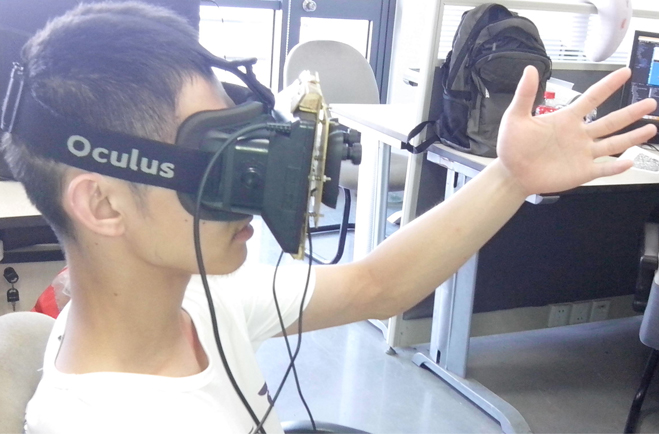
\includegraphics[height=0.2\textheight]{chap4/three-action-l1}}}
	\subfigure{\label{fig:threeaction:b}}\addtocounter{subfigure}{-2}
	\subfigure[Menu gesture in ARGlasses]{\subfigure[场景菜单手势]
		{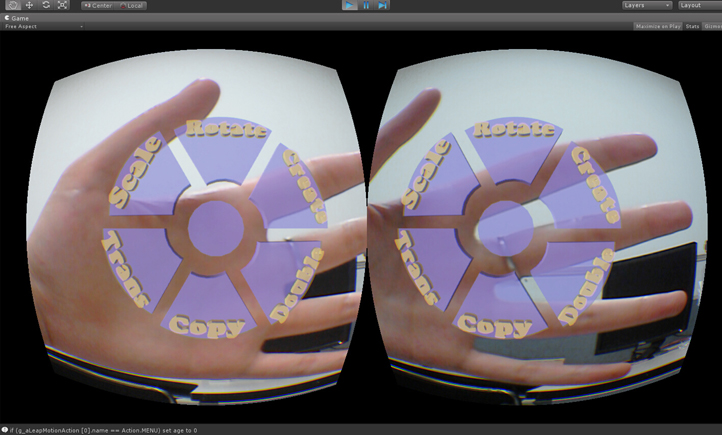
\includegraphics[height=0.2\textheight]{chap4/three-action-r1}}}
	\vspace{-1em}
	
	\subfigure{\label{fig:threeaction:c}}\addtocounter{subfigure}{-2}
	\subfigure[Selection gesture of user]{\subfigure[真人选择手势]
		{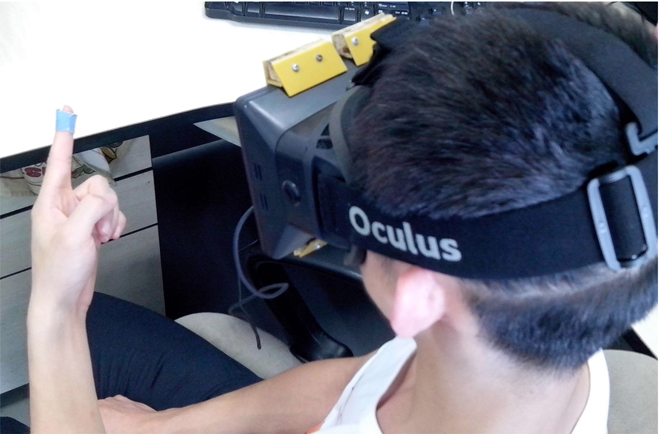
\includegraphics[height=0.2\textheight]{chap4/three-action-l2}}}	
	\subfigure{\label{fig:threeaction:menu}}\addtocounter{subfigure}{-2}
	\subfigure[Selection gesture in ARGlasses]{\subfigure[场景选择手势]
		{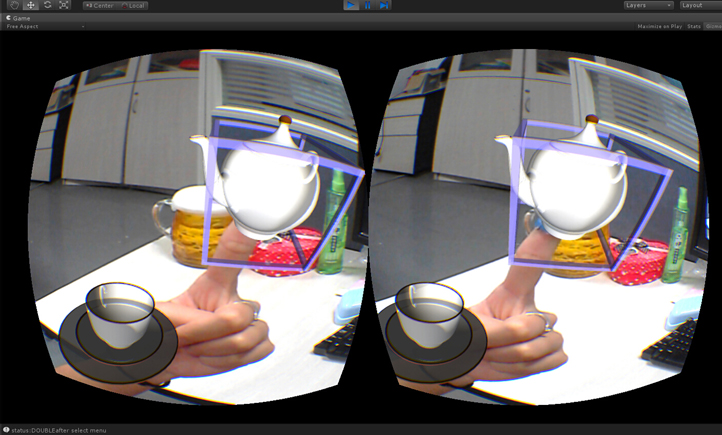
\includegraphics[height=0.2\textheight]{chap4/three-action-r2}}}
	\vspace{-1em}
	
	\subfigure{\label{fig:threeaction:e}}\addtocounter{subfigure}{-2}
	\subfigure[Manipulation gesture of user]{\subfigure[真人操控手势]
		{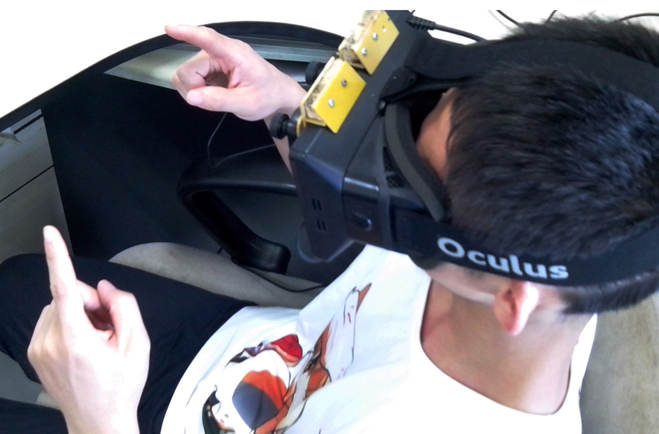
\includegraphics[height=0.2\textheight]{chap4/three-action-l3}}}
	\subfigure{\label{fig:threeaction:f}}\addtocounter{subfigure}{-2}
	\subfigure[Manipulation gesture in ARGlasses]{\subfigure[场景操控手势]
		{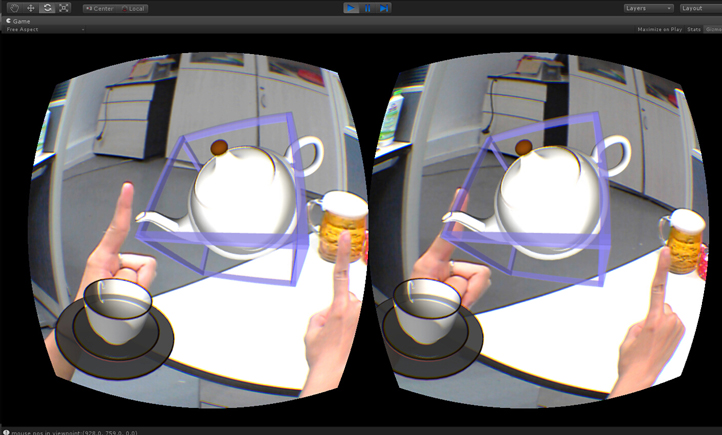
\includegraphics[height=0.2\textheight]{chap4/three-action-r3}}}
	\bicaption[fig:threeaction]{手势实景一览}{手势实景一览}{Fig.}{Three gestures in real scene}
	\vspace{-1em}
\end{figure}

\section{本章小结}
本章承接前一章的设计原则设计了用户在混合现实眼镜下的交互方式。出于学习与记忆的考虑,本文系统一共设计如图所示\ref{fig:threeaction}三个手势:菜单手势、选择手势和操控手势。
并简要介绍每个手势的设计思想和实现方法。
菜单手势由画家与调色盘的寓意而来。
选择手势沿用最通用的点击姿势,并由于硬件设备当时的融合原因增加了色环的设计,同时结合色环的设计配合\ref{sec:related-zhuangtai}节提到的状态切换的考虑,设计了选择手势与其他手势间的逻辑。
操控手势分成单双手分别介绍其交互细节与实现算法。
而后列举了在实验评估后增补的修改设计,分别是用于提醒用户当前指令的顶置提示板,提示用户手部骨骼的骨骼小球和配合手掌召唤式菜单用于工作空间分离减少误操作的头部约束。而对所有的交互设计都将在第\ref{chap:exp}章中详细评估。
%%==================================================
%% chapter03.tex for SJTU Master Thesis
%% Encoding: UTF-8
%%==================================================

\chapter{混合现实眼镜下的徒手三维建模}
\label{chap:3DModel}
本章介绍本文所设计的系统的第三个部分,通过对\ref{sec:related-cur}节中的三维建模现状及双手交互设计原则总结,设计适合混合现实眼镜场景的三维建模方法。
首先从改善双手交互的三条设计原则出发,然后为了帮助用户既保留一定的自由度,又能一定程度地优化所创建的模型弥补不同人群之间绘图技能的差异,提出自由虚拟网格平面这一想法。
自由虚拟网格平面不仅可以辅助用户创作,同时也表达了一个工作空间的概念,因而可以分离正在创作和纯移动光标两种行为。
接着阐述为了减少对整体创作过程的中断,而设计的双手职责分离概念,帮助用户在切换工具途中无缝连接前后的建模过程。
最后展示了三维建模应用场景的实现。

\section{双手交互设计原则}

首先,根据\ref{sec:related-shou}节中提到的双手交互设计三项原则,本文所设计的系统根据独有的硬件环境和应用需求做了重新评估。

%\subsection{设计原则一:保持由右及左}
\begin{enumerate}
\item 保持由右及左 \hfill\\
第一条为由右及左。本文所设计的系统维持该项原则,更精确地说,维持惯用手进行精确性操作而费惯用手进行控制类对精度要求偏低的操作。

%\subsection{设计原则二:对称的移动规模}
\item 对称的移动规模 \hfill\\
第二条原本是不对称的移动规模。本文所设计的系统将左右双手的工作空间放置在同一片区域下,因而无法也不需要对移动规模进行对应处理。
特别针对基本的物体创建,并不涉及到大规模的移动操作,于是决定采用对称的移动规模设计。

%\subsection{设计原则三:右手先行}
\item 右手先行 \hfill\\
第三条原本是左手先行,而我们采用了右手先行的原则,主要是出于对特定应用环境的考虑。
当用户在三维空间内建模时,具体在什么位置进行建模只有用户开始创建物体之后才能得知。而我们的设计是由用户使用惯用手先确定建模的初始位置,即工作空间,而后用户使用同一只手立刻进行建模,也因此保证了用户可以大致估测自己的工作空间,在想要建模的时候进入该空间范围而在不想建模的时候避开工作空间。
如果维持左手先行的原则,当交换双手时,极有可能用户会丢失自己对工作空间的概念,因而导致无法自如地建模。

\end{enumerate}
\section{自由虚拟网格平面}

自由虚拟网格平面的设计由H{\"u}rst等人\upcite{TrackingBased}启发,在其工作中提到了虚拟网格平面。
但该虚拟网格平面依附所建模物体的表面而形成,于是对于用户想要的斜面或弧度是有限制的,同样限制的还有网格的大小,于是用户只能建模一种颗粒度的物体,影响了模型的多样性。
并且由于通过移动设备(手机)才能看到建模结果,手眼之间的一致性困扰了用户的观察和理解。
同时在建模过程中,每次切换工具都会打断建模过程,非常不友好。
于是本文所设计的系统在虚拟网格平面的设计上增加了更多的自由度与操作性,提出了自由虚拟网格平面。
自由虚拟网格平面可以由用户控制它的网格大小与网格朝向,弥补前人工作的不足。

\subsection{待解决的问题}

创建物体用例有两个难点需要考虑,首先是给与用户足够的自由度进行绘制,这也是我们放弃导入模型以及使用预定义组件的原因,仅仅让用户用自己的双手进行绘制。
另一个难点是如何优化用户绘制的结果。整个应用是面向各色人群的,所以大家的绘制水平差别很大,而保证一定的绘制结果质量则是本应用设计的特色之一。
于是我们需要约束用户的绘制。
除此之外如何区分是否处在点击的状态也将在这个设计中说明。

\subsection{解决方案}

\begin{figure}[!htp]
  \centering
  \includegraphics[width=0.4\textwidth]{chap5/fvg-show}
  \hspace{1em}
  \includegraphics[width=0.4\textwidth]{chap5/fvg-show2}
  \bicaption[fig:FreeVirtualGrid]{自由虚拟网格平面}{自由虚拟网格平面}{Fig.}{Free Virtual Gird}
\end{figure}

利用辅助网格进行建模其实在各桌面建模软件中屡见不鲜,通过此类标尺一样的物体进行规范化设计的想法也深入人心。然而这样的辅助网格是否在混合现实眼镜的环境下适用得当仍未可知。因此本文所设计的系统将在此处设计一个自由的虚拟网格平面用于辅助混合现实眼镜下的三维建模。

首先,如何确定该网格平面。其创建方法如图\ref{fig:FreeVirtualGrid}所示,用户将右手自然张开伸直手指显示在眼镜前方,眼镜判断手指与掌心是否出现在同一个平面内,然后根据手掌的位置与朝向决定整个自由虚拟网格平面的位置与朝向。这个初始化操作只有在本文系统最开始运行的时候才能进行,一旦用户的手掌脱离了一个平面的约束,该网格平面便不会在随之而变动,之后也不会随用户控制变化,只会在创建模型相关的控制命令下变动。从图\ref{fig:FreeVirtualGrid}可以看到用户可以保持召唤姿势对该网格平面进行调整直到将其放置在一个合适的位置与角度下,而后所有的操控都将在这个工作环境内进行。

接下来,确定了网格平面后,该网格平面有以下两种模式供用户进行整个建模工作:涂鸦模式和拉伸模式。

%\begin{itemize}
%\item 涂鸦模式
\subsection{涂鸦模式}
\label{sec:drawMode}

\begin{figure}[!htp]
	\centering
	\subfigure{\label{fig:sketchMode}}\addtocounter{subfigure}{-2}
	\subfigure[Sketch mode in Free Virtual Gird]{\subfigure[自由虚拟网格设计中的涂鸦模式]
		{\includegraphics[height=0.25\textheight]{chap5/fvg-draw}}}
	%\vspace{-1em}
	\subfigure{\label{fig:extrudeMode}}\addtocounter{subfigure}{-2}
	\subfigure[Extrude mode in Free Virtual Gird]{\subfigure[自由虚拟网格设计中的拉伸模式]
		{\includegraphics[height=0.25\textheight]{chap5/fvg-extrude}}}
	\bicaption[fig:mode]{自由虚拟网格设计中的绘制与拉伸模式}{自由虚拟网格设计中的绘制与拉伸模式}{Fig.}{Sketch mode and extrude mode in Free Virtual Gird}
\end{figure}

%\begin{figure}[!htp]
  %\centering
  %\includegraphics[width=0.5\textwidth]{chap5/fvg-draw.jpg}
  %\hspace{1em}
  %\includegraphics[width=0.3\textwidth]{chap5/testjpg}
  %\bicaption[fig:sketchMode]{自由虚拟网格设计中的涂鸦模式}{自由虚拟网格设计中的涂鸦模式}{Fig.}{Sketch mode in Free Virtual Gird}
%\end{figure}

涂鸦模式用于让用户绘制控制点。
用户伸出一根食指触发该模式。
涂鸦模式下,用户可以在自由虚拟网格平面上绘制他想要的二维图形,而本文系统会根据用户的指尖位置和该网格平面的所有交叉点进行计算。
如图\ref{fig:sketchMode}将所示,用户所有的绘制点都对齐到该网格平面的交叉点上,于是用户可以通过该设计简单轻松地进行直线,矩形等图元的绘制,而这也是保证用户绘制质量的重要因素。
如果指尖距离网格平面太远,则视为非工作空间的操控,将不会发生任何变化。
如公式\ref{eq:drawPoint}表示的一样,对用户发出指令的点进行X轴的比较,判断是哪个控制点,同理公式\ref{eq:drawPoint2}判断Y轴的情况,然后如果Z轴方向相去甚远则视为工作空间外的干扰因素,如公式\ref{eq:drawPoint3}所计算的一样。
自由虚拟网格平面将整个空间分成了三个部分,工作环境和被分开的另两个区域
也就是凭借这一点,用户可以将之前提到的移动操作和拖拽操作区分开。

\begin{equation}
\label{eq:drawPoint}
|pos_x - crossPos_x| < 0.3
\end{equation}
\begin{equation}
\label{eq:drawPoint2}
|pos_y - crossPos_y| < 0.3
\end{equation}
\begin{equation}
\label{eq:drawPoint3}
|pos_z - virtualPlane| < 1
\end{equation}

%\item 拉伸模式
\subsection{拉伸模式}
\label{sec:extrudeMode}

%\begin{figure}[!htp]
  %\centering
  %\includegraphics[width=0.5\textwidth]{chap5/fvg-extrude}
  %\hspace{1em}
  %\includegraphics[width=0.3\textwidth]{chap5/testjpg}
  %\bicaption[fig:extrudeMode]{自由虚拟网格设计中的绘拉伸模式}{自由虚拟网格设计中的拉伸模式}{Fig.}{Extrude mode in Free Virtual Gird}
%\end{figure}

拉伸模式用于让用户将二维图形拓展至三维物体。
用户伸出至少三根手指激活该模式。
拉伸模式下,用户可以选定所需的控制点,对原有的模型,二维或者三维,进行垂直于网格平面的拉伸。
如图\ref{fig:extrudeMode}所示,被选中的点将会在网格平面的法向方向延伸,可以正向法向也可以反向,本文系统都是支持的。除了最初的二维图形绘制外,一旦物体被拉伸后,就将一直作为一个三维模型存在,用户可以继续建模。
不断重复涂鸦模式和拉伸模式可以创建出复杂的模型来。

除了基本的操作以外,本文所设计的系统提出的自由虚拟网格平面可以在最开始的初始化之后调整自身的配置,这也就是它被命名为“自由”的原因。

目前支持的调整包括朝向的调整和精度的调整。

\begin{figure}[!htp]
  \centering
  \includegraphics[width=0.4\textwidth]{chap5/fvg-rotate1}
  \hspace{1em}
  \includegraphics[width=0.4\textwidth]{chap5/fvg-rotate2}
  \bicaption[fig:rotation]{自由虚拟网格设计中的朝向调整}{自由虚拟网格设计中的朝向调整}{Fig.}{Rotation in Free Virtual Gird}
\end{figure}

\subsubsection{朝向调整}
%\begin{description}
%\item[朝向调整]\hfill\\
自由虚拟网格平面的设定是拉伸只能沿该网格平面的法向量,因而在用户进行拉伸操作时,旋转该网格平面可以使用户的拉伸方向同时得到调整,于是可以更轻松简单地创建弯折的物体。比如拱桥,比如埃菲尔铁塔。
如图\ref{fig:rotation}所示,可以看到旋转过后自由虚拟网格平面带来了模型的弯曲。

%\textbf{旋转过后的控制点如何计算的公式过程}

\begin{figure}[!htp]
  \centering
  \includegraphics[width=0.4\textwidth]{chap5/fvg-scale1}
  \hspace{1em}
  \includegraphics[width=0.4\textwidth]{chap5/fvg-scale2}
  \bicaption[fig:scalescale]{自由虚拟网格设计中的精度调整}{自由虚拟网格设计中的精度调整}{Fig.}{Scale in Free Virtual Gird}
\end{figure}

\subsubsection{精度调整}
%\item[精度调整]\hfill\\
除此之外自由虚拟网格平面在初始化之后仍旧可以调整网格的每个单元大小,所以模型的精度也可以在创建过程中变化。于是创建原型也变得可能,而有些粗颗粒度的物体则可以更简单的绘制而不需要用户对每个过程点进行劳心。
如图\ref{fig:scalescale}所示,可以看到一个棱台一样形状的物体,同样建模软件如3DMAX进行绘制,必须在选中绘制棱台的命令下才可以从底座开始绘制,然后高度,最后调整棱台的上台面。

%\end{description}

\section{职责分离的双手}

本文所设计的系统设计职责分离的双手首先为了体现混合现实眼镜的优势,该设备释放双手,所以如果能使用两只手同时进行交互是非常有利的,并且两只手完成的任务不一样,有协作有并发更可以体现该系统的高效。
另一点也是考虑到惯用手和非惯用手本就不该是一样的设计,如果将不同的职责分派下去是否会有更好的效果,这点也将在之后的评估着重讨论。

\subsection{待解决的问题}

对于专业建模软件不易于使用的一个原因是庞大的操作数量令人眼花缭乱,经常只是看着工具栏就已迷失。而另一个原因则是每次用户需要切换工具或其他命令时,必须要中断当前的建模过程,去工具栏中寻找合适的指令,而每次用户将注意力转移到工具栏或菜单栏后,整个建模的用户体验就已经被影响了。就如同\ref{sec:related-zhuangtai}节提到的一样,如何在状态切换的同时保证其显见性和平滑自然地维持整个用户体验,是很重要的。

\subsection{解决方案}

为此本文系统设计了一种方法让用户在建模途中可以在不同状态间切换同时不打断建模过程。该方法主要通过给用户的惯用手和非惯用手赋予不同的职责实现。
对于标准的单手输入设备比如鼠标,用户是很难同时进行多项任务的。
而在本文系统的设计中,利用混合现实眼镜释放双手的特性,用户可以同时使用用户的两只手进行更便捷的设计,从而创建更复杂的模型。
接下来以右手为惯用手进行阐述。
本文系统将右手设定为绘制之手,顾名思义,用户将使用且仅使用这只手进行绘制,之前\ref{sec:drawMode}节和\ref{sec:extrudeMode}节提到的绘制控制点和拉伸模型都是由绘制之手进行完成的。
它的主要职责在于创造。
而左手默认作为非惯用手,在本文所设计的系统中设定为控制之手。
负责控制当前场景的状态以及切换命令,关键在于,用户无需将绘制之手移除场景而使用控制之手进行操控,左手和右手是可以同时工作的。
目前本文所设计的系统支持两种指令:旋转和放缩。

\begin{figure}[!htp]
  \centering
	\subfigure{\label{fig:ctrl:1}}\addtocounter{subfigure}{-2}
	\subfigure[Manipulation gesture of control hand sample one]{\subfigure[控制之手的操控手势示例一]
		{\includegraphics[height=0.25\textheight]{chap5/axis-z}}}
	\subfigure{\label{fig:ctrl:2}}\addtocounter{subfigure}{-2}
	\subfigure[Manipulation gesture of control hand sample two]{\subfigure[控制之手的操控手势示例二]
		{\includegraphics[height=0.25\textheight]{chap5/rotate-grab}}}
  \bicaption[fig:ctrl]{控制之手的操控手势}{控制之手的操控手势}{Fig.}{Manipulation gesture of control hand}
\end{figure}
如图\ref{fig:ctrl}所示为操控之手的控制手势,左手自然伸出一根食指,分别对旋转的工具或放缩的工具进行操作,而图\ref{fig:switch}则是对两个操控工具的切换,切换之前如图\ref{fig:switch}(a)所示为旋转工具,而切换之后如图\ref{fig:switch}(b)所示为放缩工具。扰动手腕自然旋转两圈则表示换下一个工具,这样的设计其一考虑转圈的动作可能会有误操作,所以数量上设定为两圈,其二考虑减少用户的注意力,无需用户进行特定位置的选中,任意区域只要检测到控制之手的切换手势就对工具栏进行切换。
\begin{figure}[!htp]
  \centering
  \subfigure{\label{fig:switch:1}}\addtocounter{subfigure}{-2}
	\subfigure[Rotation tool]{\subfigure[旋转工具]
		{\includegraphics[width=0.3\textwidth]{chap5/axesInLeft}}}
	\subfigure{\label{fig:switch:2}}\addtocounter{subfigure}{-2}
	\subfigure[Scale tool]{\subfigure[放缩工具]
		{\includegraphics[width=0.3\textwidth]{chap5/scaleInLeft2}}}
  \bicaption[fig:switch]{控制之手的切换手势}{控制之手的切换手势}{Fig.}{Switch gesture of control hand}
\end{figure}

与此同时,当屏幕左方象征着工具栏的物体有了变化,如坐标轴被用户旋转后,右方的自由虚拟网格平面也会随之而旋转。
由于常见的旋转操控通常都是复杂不直观。这里本文所设计的系统采用了代理来简化旋转操作。
一共需要两步完成操作:
\begin{enumerate}[1]
\item	%\hfill \\
用户用食指抓住坐标轴中的任何一根轴的轴尖,如图\ref{fig:rotate}(a)所示
\item	%\hfill \\
用户对轴进行拖拽,坐标轴的原点不会变动,其效果和把住一个实物进行旋动的效果一致,图\ref{fig:rotate}(b)可见将X轴向上拖拽达到绕Z轴逆时针旋转的效果,可以看到图中除了坐标轴进行了这样的变化,右方的自由虚拟网格平面也进行了相同的变化。
\end{enumerate}

\begin{figure}[b]
  \centering
  \subfigure{\label{fig:rotate:1}}\addtocounter{subfigure}{-2}
	\subfigure[Before rotation]{\subfigure[旋转前]
		{\includegraphics[height=0.25\textheight]{chap5/axis-x}}}
	\subfigure{\label{fig:rotate:2}}\addtocounter{subfigure}{-2}
	\subfigure[After rotation]{\subfigure[旋转后]
		{\includegraphics[height=0.25\textheight]{chap5/axis-x2}}}
  \bicaption[fig:rotate]{旋转网格平面示例}{旋转网格平面示例}{Fig.}{Rotate free virtual grid}
\end{figure}

\begin{figure}[!htp]
  \centering
   \subfigure{\label{fig:moreRotate:1}}\addtocounter{subfigure}{-2}
	\subfigure[Rotate through axis x]{\subfigure[拖拽X轴旋转]
		{\includegraphics[height=0.18\textheight]{chap5/axis-x2}}}
	\subfigure{\label{fig:moreRotate:2}}\addtocounter{subfigure}{-2}
	\subfigure[Rotate through axis y]{\subfigure[拖拽Y轴旋转]
		{\includegraphics[height=0.18\textheight]{chap5/axis-y2}}}
		\subfigure{\label{fig:moreRotate:3}}\addtocounter{subfigure}{-2}
	\subfigure[Rotate through axis z]{\subfigure[拖拽Z轴旋转]
		{\includegraphics[height=0.18\textheight]{chap5/axis-zz2}}}
  \bicaption[fig:moreRotate]{旋转网格平面更多示例}{旋转网格平面更多示例}{Fig.}{Different types of rotation}
\end{figure}

为了更清楚地说明旋转原理,图\ref{fig:moreRotate}展示了抓住三根轴往三个标准方向旋转的事例。分别是抓住X轴上下拖拽来绕Z轴旋转(见图\ref{fig:moreRotate}(a));抓住Y轴前后拖拽来扰X轴旋转(见图\ref{fig:moreRotate}(b));和抓住Z轴左右拖拽来扰Y轴旋转(见图\ref{fig:moreRotate}(c)),坐标轴的变化和一边自由虚拟网格的变化都清晰地展示了效果。
而操控之手的旋转操作,详情见算法\ref{alg:model:rotate}:

	\begin{algorithm}  
		\caption{操控之手的旋转操作算法}  
		\label{alg:model:rotate} 
		\begin{algorithmic}  
		\REQUIRE{虚拟网格平面针对被选中的轴$Axis$和移动距离$projectLength$}
		\ENSURE{更新后的控制点$SET_c_p$}
			\STATE{将$Axis$根据$projectLength$进行旋转}
			\STATE {得到所有控制点$SET_c_p$}   
			\FOR{each $cp_c_o_o_r_d \in SET_c_p$}
				\STATE{计算世界坐标系下相对于网格平面的坐标\\$cp=cp_c_o_o_r_d*S_p_l_a_n_e*S_s_q_u_a_r_e$}
				\STATE{计算世界坐标系下的坐标\\$cp_w_o_r_l_d=transform.transformPoint(cp_w_o_r_l_d)$}
			\ENDFOR
		\end{algorithmic}  
	\end{algorithm} 

%\begin{figure}[!htp]
  %\centering
  %\includegraphics[width=0.3\textwidth]{chap5/testpng}
  %\hspace{1em}
  %\includegraphics[width=0.3\textwidth]{chap5/testjpg}
  %\bicaption[fig:scale]{缩放网格平面}{缩放网格平面}{Fig.}{Zoom in or out}
%\end{figure}

缩放手势则针对缩放工具倒圆锥进行,当用户的操控之手触及倒圆锥时,自由虚拟网格平面的单元大小就和倒圆锥上用户的手指位置绑定在了一起。用户在倒圆锥上进行上下移动会导致该网格平面变大或者变小,当用户的操控之手脱离倒圆锥时,操控自然停止,类似一个自动触发的滚动条。
	
为了保证缩放前后用户所建模型的相对位置不受变化,
\begin{algorithm}  
		\caption{操控之手的放缩操作算法}  
		\label{alg:model:scale} 
		\begin{algorithmic}  
		\REQUIRE{控制点$SET_c_p$,虚拟网格平面放缩因子$S_p_l_a_n_e$,网格大小$S_s_q_u_a_r_e$}
		\ENSURE{更新后的控制点$SET_c_p$}
			\FOR {each point $p_c_o_o_r_d \in SET_c_p$}
				\STATE{累加$p_c_o_o_r_d$求和}
				\STATE{计算世界坐标系下相对于网格平面的坐标\\$p=p_c_o_o_r_d*S_p_l_a_n_e*S_s_q_u_a_r_e$}
				\STATE{计算世界坐标系下的坐标\\$p_w_o_r_l_d=transform.transformPoint(p_w_o_r_l_d)$}
			\ENDFOR
			\STATE{平均求得中心点的坐标$pCenter_c_o_o_r_d$}
			\STATE{计算世界坐标系下相对于网格平面的坐标\\$pCenter$ 和$pCenter_o_l_d$}
			\FOR{each $p_w_o_r_l_d$}
				\STATE{将$p_w_o_r_l_d + pCenter - pCenter_n_e_w$加入控制点集合$control points$}
			\ENDFOR
		\end{algorithmic}  
\end{algorithm} 
因而系统此处默认采用中心放缩的方法,中心为用户所创建的模型在网格平面上的中心,具体算法见算法\ref{alg:model:scale}:	

\section{三维建模应用场景实现}
在设计了自由虚拟网格平面用以辅助用户绘制,及职责分离的双手原则来无缝连接建模过程中的状态切换后,接下来将描述本文系统针对的徒手三维建模场景。

\begin{figure}[!htp]
	\centering
	\subfigure{\label{fig:model:1}}\addtocounter{subfigure}{-2}
	\subfigure[House with the pinnacle]{\subfigure[尖顶房屋]
		{\includegraphics[height=0.3\textheight]{chap6/house}}}
	\subfigure{\label{fig:model:2}}\addtocounter{subfigure}{-2}
	\subfigure[House with flat roofs]{\subfigure[平顶房屋]
		{\includegraphics[height=0.3\textheight]{chap6/house-2}}}
	\bicaption[fig:model:house]{建模场景之房屋}{建模场景之房屋}{Fig.}{Houses in model application}
	\vspace{-1em}
\end{figure}

\subsection{应用简介}
徒手三维建模场景是在任意场景下,用户戴上系统配置的混合现实眼镜,不佩戴任何其他辅助工具进行双手建模的应用场景。
针对本文系统设计的三维建模特点,本应用特对设计了以下三个建模目标进行效果展示。
\begin{enumerate}
\item 基本房屋\hfill\\ 
一个基本的房屋必须有一个柱形的房屋本体,通常以方形为主,不规则多边形亦是一种选择,而后如果是一幢独立房屋则会有一个屋顶,以尖顶居多,平顶也是一种常见设计。
\item 艺术花瓶\hfill\\ 
一个艺术花瓶整体形状将呈现一个柱形,但在柱形区域的横截面通常为不同半径的圆盘,否则其将不为一个花瓶而只是一个圆柱体罢了,通过半径的调整将展现自成一脉的艺术花瓶。
\item 一座拱桥\hfill\\ 
一座拱桥的整体构架是一个半圆,或高或低的半圆皆可,而这座半圆始末为拱桥的桥墩,通常桥墩形状为长方形,其他的形状亦可。
\end{enumerate}

用户将通过以上三种建模目标感受自由虚拟网格及职责分离原则的设计。

\subsection{效果展示}

图\ref{fig:model:house}显示了一个基本房屋。用户创建了方形的底座,从图上可以看到黄色的控制点,然后向上拉伸,接着选中方形拉伸区域内靠中间的控制点,进行第二次拉伸,于是完成了图\ref{fig:model:house}(a)中所见的尖顶,如果拉伸时选中两个点将会产生平顶效果,如图\ref{fig:model:house}(b)所示。
此处建模房屋只需要使用绘制之手的涂鸦模式和拉伸模式,简单易行。

\begin{figure}[t]
  \centering
  \includegraphics[width=0.4\textwidth]{chap6/vase}
  \bicaption[fig:model:vase]{建模场景之花瓶}{建模场景之花瓶}{Fig.}{Vase in model application}
\end{figure}

图\ref{fig:model:vase}显示了一个艺术花瓶。可以看到艺术花瓶最开始由底部平稳拉伸向上,而后采用控制之手切换工具调整网格大小,于是花瓶的半径开始变小,
而在调整大小的操控环境下,用户的操控之手离开倒圆锥工具,此时便无法调整半径大小,于是绘制之手又可以将花瓶平稳向上拉伸,也就是后三分之一阶段花瓶半径保持不变的功效。此处需要结合操控之手和绘制之手共同完成协作,而在工具切换时从来不需要绘制之手放下或者等待,因为建模的流程从未中断。

\begin{figure}[t]
  \centering
  \includegraphics[width=0.4\textwidth]{chap6/bridge}
  \bicaption[fig:model:bridge]{建模场景之拱桥}{建模场景之拱桥}{Fig.}{Bridge in model application}
\end{figure}

图\ref{fig:model:bridge}显示了一座微微弯曲的拱桥。用户首先创建了一个长方形的桥墩,桥墩面积并不大,也给之后的旋转拉伸提供了空间。
而后用户将桥墩慢慢上拉,并同时用操控之手选中坐标轴工具中的Y轴,将Y轴向左拖拉,从而达到整个网格平面沿Z轴顺时针旋转的效果。
于是桥墩在向上的同时开始向右旋转,同时进行着旋转和拉伸可以看到桥墩缓缓向左方延伸。
直到最后形成一个微微弯曲的拱桥。

通过图\ref{fig:model:house}、图\ref{fig:model:vase}和\ref{fig:model:bridge}可见在重新设计的双手交互原则、自由虚拟网格的辅助及职责分离的思想支持下,用户可以简单地创作一些相对复杂的三维模型,而针对三维模型的效果、时间开销等可行性与易用性的评估将会在下章详细描述。

\section{本章小结}

本章具体介绍了混合现实眼镜下的徒手建模设计。
首先确定了本文所设计的系统采用的双手交互原则,将前人的工作和本文所设计的系统所处的硬件与应用环境结合得到适合的新原则。
然后提出本文所设计的系统对于三维建模应用的第一个新方法,自由虚拟网格平面。
与前人工作中提到的虚拟网格平面不同在于其自由度,其一为可以在初始化配置后进行朝向的旋转,其二为单元格大小的调整,于是可以支持弯曲的和精度不同的模型建设,仅是这两点就可以创建复杂的模型了。
不仅如此,自由虚拟网格平面解决了一部分的状态切换问题,通过自由虚拟网格平面的提示,用户清晰地知道自己的工作环境,因而不会有单纯的手指移动导致对模型的误操作,系统会判断当前手指是否在工作环境平面内。
接着提出了第二个辅助建模工作的方法,双手职责分离。为了突出混合现实眼镜释放双手的特性并扩大双手操作的益处,本文所设计的系统给惯用手和非惯用手安排了不一样的任务,一则负责精细具体的绘制,一则负责偏控制的命令操作。
并对其中涉及的算法都予以简单概述。
最后展示了通过以上设计展开的三维建模应用场景效果,通过基本房屋、艺术花瓶和拱桥三个建模目标体现了本文系统所设计的徒手三维建模方法能的实用性。
%%==================================================
%% chapter03.tex for SJTU Master Thesis
%% Encoding: UTF-8
%%==================================================

\chapter{实验与评估}
\label{chap:exp}

本章将描述本文系统设计的所有实验。
本文针对所设计的系统中每一个设计都进行了非项目参与人员的用户调研,分别是对三维菜单与操控手势的可行性评估,对单手操控、双手操控和辅助设计的易用性评估,
对空间设计基本操控的初步评估以及对用户进行具体建模要求的正式评估。
实验评估项目由用户的主观问答得分和被记录的客观时间次数参数组成。
从评估结果可见,混合现实眼镜下的三维界面、交互手段与徒手三维建模场景都具有一定的可行性与易用性。

\section{三维菜单与三维操控的可行性评估}
\label{sec:exp:feasibility}
首先,针对混合现实眼镜下的手势交互和菜单设计进行可行性评估。
\subsection{实验介绍}
开始,我们先给五位实验者(最小年龄 22 岁,最大年龄 25 岁,平均 23.4岁)简单介绍了本文系统,并展示了基本操控。实验者在此之前对该系统并无了解,也从未接触过 Oculus VR和 Leap Motion。然后开始训练,训练分为以下几步:
\begin{enumerate}
\item 使用菜单手势调用手掌召唤式菜单创建物体
\item 使用目标跟踪式菜单旋转物体
\item 使用屏幕固定式菜单放缩物体
\end{enumerate}

训练过后,实验者对本文系统有了初步的了解,开始正式实验任务。共有三个实验,实验步骤一致,但分别采用三种不同的菜单(手掌召唤式菜单、目标跟踪式菜单和屏幕固定式菜单)。实验步骤如下:

\begin{enumerate}
\item 在不同位置分别创建一个茶壶和一个茶杯
\item 使用单手操控将茶壶放置到茶杯的附近,呈现倾倒的状态
\item 使用双手操控将茶杯杯口向上
\item 拷贝这套茶具
\end{enumerate}

统计所得训练时间从 6 到 11 分钟不等,而完成三个实验总共需要 20 分钟左右。实验结束后,每个实验者都需完成一份调查问卷。

\subsection{可行性实验结果与分析}
\label{subsec:exp:feasibility}

\begin{figure}[!htp]
  \centering
  \includegraphics[width=0.8\textwidth]{chap6/eva-feasibility}
  \bicaption[fig:feasibility]{三维菜单与三维操控的可行性分析问卷}{三维菜单与三维操控的可行性分析问卷}{Fig.}{The feasibility questionnaire of 3D menus and 3D manipulation}
\end{figure}

所有的实验参与者都完成了训练,只有一个人在第四项实验任务中失败了。实验过程中我们发现参与者在操控方面都碰到了困难,一方面是从未使用过 Leap Motion,无法十分熟练地使用 Leap Motion,另一方面当物体没有按照参与者的预料变化时,参与者不知道应该如何处理,关于加强 Leap Motion 的操控方面,训练和更多的系统提示都是必要的。
这也就是后来在\ref{sec:interaction:skeleton}节中提到的骨骼小球增加的原因。

根据大家的问卷调查,我们得到了如图\ref{fig:feasibility}所示的可行性结果分析。参与者对所有项目进行打分,0 分为最低分表示最不认同,10 分为最高分表示最为认同。

首先评估本文系统设计的三种菜单(手掌召唤式菜单、物体跟踪式菜单和屏幕固定式菜单)。虽然三类菜单的得分互相间略有差异,但与操控物体类的得分相比都属偏高,说明触发菜单指令比操控物体更容易。有时由于过于灵敏,用户可能无意中做出菜单手势触发了菜单。而这个过于触发的误操作也就是\ref{sec:interaction:head}节提到的头部约束设定的来源。

其次评估选择操作。大多数参与者都表示可行,只有一个参与者遇到了困扰。其在实验中带着色环对物体进行操控时,物体没有随着手的变化而变化,因为带着色环是不能对物体进行操控操作的。当用户理解了本文系统在选择物体和操控物体的状态切换原则后,就消除了困惑。此外,由于选择菜单后,菜单消失的同时,菜单操作区域和物体操作区域可能重叠,导致实验者无意中选中物体。同时,有参与者提出,如果能在选中菜单后有更明显的状态提示,会更了解当前系统的情况。也是因此设计了\ref{fig:interaction:board}节提到的顶置提示板。

最后是操控类评估,单手操控物体的得分远大于双手操控。
原因有二,其一是单手操控的设计接近触摸屏的操作,参与者很快就熟悉了起来,而且表示不用一直拿着手机或者平板感觉轻松不少;
其二是双手操控物体时,常常因为距离或者角度的原因超过了 Leap Motion 的接收范围,以至于无法成功操作。此外,无论是单手还是双手操控,参与者都表示很难进行特别精细的操作,诸如旋转 90°,放大成原来的 2 倍等。

\section{三种菜单的偏好布局分析}

\subsection{实验介绍}
本次实验共有两个部分,一则比较不同的布局,一则比较批处理操作时大家喜好是否会有变化。实验邀请了 10 位志愿者,其中 8 位男生,2 位女生,实验任务介绍如下:
\begin{enumerate}
\item 实验者通过目标物系列菜单进行虚拟物体创建并缩放。目标物系列菜单为目标跟踪式菜单和屏幕固定式菜单,而在这项任务完成后对二者进行选择。
\label{exp:object-series}
\item 实验者使用完成实验\ref{exp:object-series}后选择的目标物系列菜单和手掌召唤式菜单分别对三个物体进行拷贝并将他们旋转至面朝右方,值得注意的是这里的具体操作流程并不一样也导致了之后实验的评估。
\label{exp:batch}

\subsection{三种菜单布局的喜好分析}
\end{enumerate}
\begin{figure}[!htp]
  \centering
  \includegraphics[width=0.8\textwidth]{chap6/preference}
  \hspace{1cm}
  \includegraphics[width=0.8\textwidth]{chap6/batch}
  \bicaption[fig:preferenceMenu]{三种菜单的偏好选择}{三种菜单的偏好选择}{Fig.}{Preference on three types of menus}
\end{figure}

本次实验的目的是为了分析三种布局的菜单在用户心中的使用偏好。
并且当任务内容发生变化时,对三种类型的菜单选择是否会有变化。

图\ref{fig:preferenceMenu}显示没有用户喜欢目标跟踪式菜单。手掌召唤式菜单的特点是永远出现在手中,随掌而动;屏幕固定式菜单的特点是永远出现在屏幕中央,大而明晰;而对于目标跟踪式菜单,虽然从语义上紧跟目标物非常合理,但由于Oculus VR目前的像素以及菜单的逻辑设定会随目标物的朝向与大小而变,导致观察菜单的难度提升,这些都是影响因素。

同时选择屏幕固定式菜单和手掌召唤式菜单的人数中,一部分实验者倾向先确定目标物,于是他们偏好屏幕固定式菜单而另一部分实验者倾向先确定操作于是他们偏好手掌召唤式菜单。
接着在批处理(即实验\ref{exp:batch}中,大部分实验者都选择了手掌召唤式菜单,因为选择该菜单可以减少完成实验任务的步骤并且每个被操作的物体都可以互相保持一致的角度,使整个任务完成的质量更好。

\section{辅助设计与单手、双手操控的易用性评估}
\label{sec:exp:usability}

为了验证新增的几项修改是否有效,我们针对改进版的系统进行了更加正式的易用性评估。评估了如下内容:

\begin{enumerate}
\item 本文系统的总体使用感受
\item 提示板、手势可视化以及结合头部的手势设计这几方面的易用性
\item 单双手操控的比较和当前系统对精确操控的支持度
\end{enumerate}

\subsection{实验介绍}
同样从系统介绍开始,展示了系统的基本操控方法后,首先开始了训练步骤:
\begin{enumerate}
\item 使用 Leap Motion 训练菜单手势和操控手势
\item 启用顶置提示板,用手掌召唤式菜单创建物体
\item 启用骨骼小球,用目标跟踪式菜单对物体进行单手旋转
\item 启用头部约束,用屏幕固定式菜单对物体进行双手操控
\end{enumerate}

训练部分完成后,用户对新增的几种修改都有了大致了解,之后便是正式的实验任务,步骤如下:
\begin{enumerate}
\item 用手掌召唤式菜单创建茶壶和茶杯,启用头部约束和关闭各一次
\item 用目标跟踪式菜单单手操控茶壶,使之呈倾倒状,启用骨骼小球和关闭各一次
\item 用屏幕固定式菜单拷贝茶壶和茶杯,启用提示板和关闭各一次
\item 指定参考茶壶 A 和茶壶 B、 C,使用单手操控将茶壶 B 调整到与参考茶壶 A 大小朝向一致,再使用双手操控将茶壶 C 同样调整一遍
\label{item:uniandbi}
\end{enumerate}

整个实验过程中对每个提示启用与否的操控都有计时,用户完成实验后进行问卷填写。

\subsection{用户的总体使用感受}

首先,用户对混合现实眼镜有较大的兴趣,觉得直接能看到增强现实的场景,而不用通过屏幕,非常地直观,在满分 10 分的总体易用性评估中获得7.5 分。
并且对表示绑定在手上的菜单感觉新奇,仿佛自身的功能得到了增强。然而当前制作的增强现实眼镜仍然不够轻便,
且 OculusVR目前像素较低,几乎所有用户都在实验完成后表示头有些重,眼睛有些不适。

其次,用户对于不用佩戴沉重设备的近乎裸手
交互也表达了支持的态度,单手操控很顺畅就像空
中有一个触摸屏,双手操控效果也很令人激动只是
不够灵敏还需要再改进。

\begin{figure}[!htp]
  \centering
  \includegraphics[width=0.8\textwidth]{chap6/fuzhu}
  %\hspace{1cm}
  %\includegraphics[width=0.3\textwidth]{chap6/testpng}
  \bicaption[fig:exp:usability]{辅助功能的易用性分析}{辅助功能的易用性分析}{Fig.}{The usability of the design for assistance}
\end{figure}

图\ref{fig:exp:usability}显示了改进版系统的易用性分析,数值表示参与实验的 10 人中愿意保留各项改进的人数。

\subsection{顶置提示板的易用性分析}
图\ref{fig:exp:usability}显示了用户对是否愿意保留提示板的看法,只有 1 名参与者表示无需提示板,感觉提示板的出现显得整个增强现实界面有点冗余,其他 9 名
参与者都支持这个新的补充。
根据表\ref{table:exp:skeleton}中记录的时间,实验任务 3 中实验者在打开提示板和关闭提示板的两种情况下,完成任务的时间基本一致。
虽然提示板没有在完成任务的效率上有明显提升,但在心理上给了用户更多的支持,值得保留。

此外,有 1 名实验者表示提示板的位置过高,注意力很难集中到视野的边缘处,关于提示板的安置位置或者变化时机,还可以做更多的改进。

\subsection{手势可视化之骨骼小球的易用性分析}

\begin{table}[!hpb]
  \centering
  \bicaption[table:exp:skeleton]{开启或关闭辅助功能的各项平均时间统计}{开启或关闭辅助功能的各项平均时间统计}{Table}{Average time consumption on enabling or disabling the assistance}
  \begin{tabular}{@{}cccc@{}} \toprule
    实验内容 & 实验1/秒 & 实验2/秒 & 实验3/秒 \\
	\midrule
    修改内容 & 头部约束 & 骨骼小球 & 顶置提示板 \\
    启动修改完成的平均时间 & 82 & 44 & 70 \\
    关闭修改完成的平均时间 & 143 & 70 & 85 \\
	\bottomrule
  \end{tabular}
\end{table}

图\ref{fig:exp:usability}显示了大家对是否愿意保留骨骼小球的看法。
多数实验者表示骨骼小球的提示是有用的,可以知道目前自己的手势是否被检测,检测的形态是什么样子,以此来调整自己的手势更好地进行操控任务。
而反对意见表示,有时候由于手势角度的原因 Leap Motion 检测到的手势比较混乱,于是整个场景就会被混乱的骨架所干扰,影响操控的效率。
1名实验者提议可以将手势骨架转化成两种文字提醒,一种提醒手势在Leap Motion检测区域内,另一种提醒超出范围以外即可。 
从表\ref{table:exp:skeleton} 的统计结果来说,启用骨骼小球在一定程度上对操控性能有所提升,值得保留。

\subsection{单手操控与双手操控的对比}
\begin{figure}[!htp]
  \centering
  \includegraphics[width=0.8\textwidth]{chap6/univsbi}
  \bicaption[fig:exp:univsbi]{单手操控与双手操控的偏好统计}{单手操控与双手操控的偏好统计}{Fig.}{Preference on unimanual interaction and bimanual interaction}
\end{figure}

实验\ref{item:uniandbi}中,参与者使用单手操控和双手操控的方法对物体进行了控制。
从图\ref{fig:exp:univsbi} 中可以看到,绝大部分用户喜欢单手操控,原因与\ref{subsec:exp:feasibility}节分析的一致。
还有用户提到,经常需要切换具体指令如单手平移等,有些不便。
而选择双手操控的 1名用户是任务完成中最快最好的,一方面无需不停地进行状态切换,一方面双手的操控和现实更为接近,十分直观。
然而在实验\ref{item:uniandbi}中,所有参与者都表示要使被操控的物体和参考物体在姿态上完全相似,非常困难,难以精细地对物体进行旋转,无论是单手操控还是双手操控,原因是操控中手部和头部的轻微移动会影响操控的效果,这也是本文系统目前的不足。

\section{空间设计的基本操控评估}
\label{sec:exp:pilot}
本次实验针对本文工作中的空间设计部分,进行混合现实眼镜下的基本操控评估。

\subsection{实验介绍}
本次实验的环境就在实验室中,完全日常的环境配备,无需特殊的调整。
参与人员由14个研究生和1个本科生组成。其中10名男生,5名女生,年龄从20到25岁不等,平均为22.8岁,标准差为1.42。
所有人的惯用手都是右手,其中9名实验者曾使用过虚拟现实或者增强现实的设备,所有人都没有参与到本文系统的设计实现中。
基本操控评估包括手势和基本功能的测试,以下为实验步骤:
\begin{enumerate}
\item 使用右手自然张开五指配置初始化的自由虚拟网格平面
\item 在指定的四个紫色点上绘制控制点
\label{exp:cp}
\item 使用切换工具的手势将旋转工具切换为放缩工具
\item 选择旋转工具中的某具体坐标轴
\end{enumerate}

以下为评估标准,一共是三项:
\begin{enumerate}
\item 执行时间(Execute Time/ET) \hfill \\
实验者在每个单项任务上所耗费的时间
\item 误操作率(Rate of Misoperation/RM) \hfill \\
用错误的次数比上全部的尝试次数。如当用户想要旋转虚拟网格平面时,错误地变换了控制工具等。这就视为一次误操作。
\item 准确率(Rate of Accuracy/RA) \hfill \\
用正确的次数比上总共尝试的次数。如要求实验者选中指定的目标物,如果指到了则视为一次正确的操作。
\end{enumerate}

\subsection{基本操控实验结果分析}

\begin{figure}[!htp]
  \centering
  \includegraphics[width=0.8\textwidth]{chap6/eva-question}
  \bicaption[fig:spcItrc:basic]{基本操控实验的问卷调查}{基本操控实验的问卷调查}{Fig.}{The questionnaire of pilot experiment}
\end{figure}

在所有的实验过程中,只有1名实验者没有完成所有的任务,究其原因因为Leap Motion设备始终无法正确捕获他的手指类别,而这一点在应用设计中是有具体对应的。
另外14个参与者都成功完成实验。
对于空间设计中的基本操控感受,每个实验者都完成了一份主管的问卷调查,显示在图\ref{fig:spcItrc:basic}中,分值从0浮动到10,分数越高越表示赞同。

%\begin{figure}[!htp]
  %\centering
  %\includegraphics[width=0.6\textwidth]{chap6/eva-fvg-call}
  %\bicaption[fig:spcItrc:initial]{设定初始自由虚拟网格平面耗时}{设定初始自由虚拟网格平面耗时}{Fig.}{Time consumption on initializing free virtual grid}
%\end{figure}

如表\ref{table:exp:initial}所示,整个实验花去用户2秒到13秒不等的时间来进行初始网格平面的调整(ET)。
之所以有部分实验者花费超过十秒的时间来设置初始设定是为了在之后的实验中获得更好的体验。
尤其当实验者能够长时间进行放置自由虚拟网格平面的操作时,也就是表明实验者对这一手势的熟悉。
没有任何一名实验者在这一任务上失败,并且从图\ref{fig:spcItrc:basic}的问卷调查中也可以看到对这一动作大家觉得很轻松。

\begin{table}[!hpb]
  \centering
  \bicaption[table:exp:initial]{完成易用性实验的平均时间统计}{完成易用性实验的平均时间统计}{Table}{Average time consumption for feasibility experiment}
  \begin{tabular}{@{}ccc@{}} \toprule
    实验者编号 & 初始化耗时/秒 & 切换工具耗时/秒\\
	\midrule
    1 & 4.5 & 4.9\\
	2 & 5.14 & 3.8\\
	3 & 4.86 & 6\\
	4 & 6.168 & 1.7\\
	5 & 4.105 & 1.6\\
	6 & 5.211 & 3.628\\
	7 & 10 & 2.21\\
	8 & 8.29 & 1.737\\
	9 & 3.8 & 1.838\\
	10 & 2.6 & 2.479\\
	11 & 8.288 & 10\\
	12 & 2.98 & 2.145\\
	13 & 4.39 & 2.628\\
	14 & 5.047 & 2.729\\
	平均值 & 5.384 & 3.386\\
	标准差 & 2.125 & 2.303\\
	\bottomrule
	%&5.14&4.86&6.168\\
	%切换工具耗时 & 4.9 & 3.8 & 6 & 1.7 \\
	  %实验单位 & 实验者5 & 实验者6 & 实验者7 & 实验者8 \\
	  %初始化耗时 &4.105&5.211&10&8.29\\
	  %切换工具耗时  & 1.6& 3.638 & 2.21 & 1.737 \\
	  %实验单位 & 实验者9 & 实验者10& 实验者11 & 实验者12 \\
	  %初始化耗时&3.8&2.6&8.288&2.98\\
	  %切换工具耗时 & 1.838 & 2.479& 10 & 2.145 \\
	  %实验单位 & 实验者13 & 实验者14 & 平均值&标准差\\
	  %初始化耗时&4.39&5.047&5.384214286 & 2.125342223\\
	  %切换工具耗时& 2.628 & 2.729 & 3.386 & 2.303924812\\
	  %\bottomrule
  \end{tabular}
\end{table}

%\begin{figure}[!htp]
  %\centering
  %\begin{subfigure}[b]{0.3\textwidth}
                %\includegraphics[width=\textwidth]{chap6/eva-fvg-circle}
                %\bicaption[fig:spcItrc:circle]{切换工具手势耗时}{切换工具手势耗时}{Fig.}{Time consumption on circle gesture}
  %\end{subfigure}
  %\hspace{1in}
  %\begin{subfigure}[b]{0.3\textwidth}
                %\includegraphics[width=\textwidth]{chap6/eva-fvg-choose-axis}
                %\bicaption[fig:spcItrc:axes]{选择坐标轴耗时}{选择坐标轴耗时}{Fig.}{Time consumption on choosing axes}
  %\end{subfigure}
  %\bicaption[fig:spcItrc:time]{切换工具手势和选择坐标轴的耗时}{切换工具手势和选择坐标轴的耗时}{Fig.}{Time consumption on circle gesture and choosing axes}
%\end{figure}

%\begin{figure}[!htp]
  %\centering
  %\includegraphics[width=0.4\textwidth]{chap6/eva-fvg-circle}
  %\hspace{1cm}
  %\includegraphics[width=0.4\textwidth]{chap6/eva-fvg-choose-axis}
  %\bicaption[fig:spcItrc:time]{切换工具手势和选择坐标轴的耗时}{切换工具手势和选择坐标轴的耗时}{Fig.}{Time consumption on circle gesture and choosing axes}
%\end{figure}

如表\ref{table:exp:initial}所示,实验者通常需要少于3秒的时间来完成切换工具的手势(ET)。
而在整个实验进行中,当实验者执行其他操作时并没有出现意外地切换工具的情况发生(RM)。
如图\ref{fig:spcItrc:axes}所示,实验者要花费更多的时间在选择坐标轴上(ET),但同样发现图\ref{fig:spcItrc:axes}中的标准差亦是很大,可见不同的实验者所需的时间差别很大,进一步了解到这同样受当前坐标轴的位置和要选择的坐标轴是哪一个有关。
当进行\ref{sec:exp:model}节的建模实验时,我们并没有发现实验者对于选择特定的坐标轴来进行旋转操作有任何困难。
除此之外,我们同样可以从图\ref{fig:spcItrc:basic}中获悉实验者在切换工具这一项上给了高分,可见这一建模方法在一定程度上还是轻松易学的。
\begin{figure}[!htp]
  \centering
  \includegraphics[width=0.9\textwidth]{chap6/selectaxes}
  \bicaption[fig:spcItrc:axes]{选择坐标轴耗时}{选择坐标轴耗时}{Fig.}{Time consumption on choosing axes}
\end{figure}

如图\ref{fig:spcItrc:selcp}所示,几乎所有的实验者都能在自由虚拟网格平面上选定给定的四个控制点(RA),其中两名实验者没有成功选择因为他们没有理解必须在几乎和自由虚拟网格平面同一个平面上进行控制点的绘制,也就是工作空间的概念。
有时实验者的手指在该网格平面的正上方,虽然看起来正指在某个控制点上,但其实尚有距离。反过来思考着一点,实验者便可以通过抬高或降低自己的手的平面来防止自己无意中对控制点的选择,减少误操作。

\begin{figure}[!htp]
  \centering
  \includegraphics[width=0.8\textwidth]{chap6/eva-select-points}
  \bicaption[fig:spcItrc:selcp]{选择指定控制点}{选择指定控制点}{Fig.}{Choosing specific points}
\end{figure}

在基本操控实验之后,实验者对与本文系统设计的空间设计也有了一定了解。整个实验的介绍约莫十分钟而整个基本操控实验耗时也接近十分钟,部分实验者对操控旋转工具非常感兴趣,甚至在实验之后继续操作了一会,也在另一角度说明本文系统提出的这一方法是很有趣的。
同时基于问卷调查的主观印象和我们记录的操作时间、误差率和准确率的客观数据,我们可以得出结论该空间设计所涉及的基本操作时简单易学的。初始化手势非常稳定,绘制手势非常直观,而切换工具手势又相当有趣,基于这样的结论我们开始了正式的建模实验。

\section{空间设计的建模评估}
\label{sec:exp:model}

\subsection{建模实验介绍}
在建模实验中,我们设计了三个具体的模型让用户创建。这些模型分别展示了本文所设计系统的不同特性,三个模型的描述与建模技巧如下:

\begin{enumerate}
\item 基本房屋\hfill\\ 实验者需要先创建一个房屋的根基,方形或其他形状皆可。通过选择用户认为所需的控制点并且沿法向拉伸构成一个房屋的主体,这时候实验者已经可以看到一个柱形,最后再选一次控制点沿同一方向拉伸出一个房屋的尖顶。
\item 艺术花瓶\hfill\\ 实验者同样需要先设计一个花瓶的底座,一般以接近圆形为主,然后确定一个拉伸的朝向。在拉伸过程中,实验者需要将工具切换成放缩工具,并操控自由虚拟网格平面的大小,无论变大还是变小均可,如此这般一个自定义花瓶诞生。
\item 一座拱桥\hfill\\ 实验者需要先创建拱桥的桥墩,多数为长方形,然后在拉伸桥墩的过程中使用操控之手对自由虚拟网格平面进行旋转,于是桥墩在拉伸的途中会沿同方向进行倾斜,最终构成一座拱桥。
\end{enumerate}

\subsection{建模实验评估}

\begin{figure}[!htp]
  \centering
  \includegraphics[width=0.8\textwidth]{chap6/eva-question-formal}
  \bicaption[fig:spcItrc:formal]{建模问卷调查}{建模问卷调查}{Fig.}{Formal experiment questionnaire}
\end{figure}

开始之前照例向实验者阐述了实验过程中要创建的三个模型,并且将模型的特性和本文系统的特性都分别予以了阐述,帮助实验者更好地理解本文系统与实验。从图\ref{fig:spcItrc:formal}中可以看到实验者对与三个模型创建的反馈。分数从0分到10分由低到高表示负面到正面的感受。首先我们可以看到拉伸手势的分数很高。每次用户创建一个三维模型都需要使用拉伸手势,也因此对于该手势的练习次数很多。同理可知对于绘制手势实验者也是较为熟悉。
%图\ref{fig:spcItrc:model}展示了部分实验者创建的模型,可以看到基本房屋的构造非常明晰,艺术花瓶的效果在变化的半径上略有体现,拱桥的弧度一样清晰可见,虽然不够大,但也是一个不错的开始。

对于三种模型的创建,我们结合用户在图\ref{fig:spcItrc:formal}的反馈中进一步分析。第一个模型是基本房屋,实验者只需要使用绘制之手(也就是惯用手)来完成该实验。大部分实验者在实验进行中要求进行多次,因为他们希望创建出不同形状的有趣的房子。其中一名实验者,没有任何使用虚拟现实或增强现实的设备经验,一共进行了四次最终绘制成功。无论如何实验者尝试建模的次数始终很小,同样表明本文系统提供的这套方法简单易上手。当实验者在创建房屋时,观察到实验者对与绘制手势的使用非常平滑自然且选择想要的控制点比在基本操控实验\ref{exp:cp}中要迅速很多。

图\ref{fig:spcItrc:time}显示了用户在创建房屋时的时间统计,观察可得时间的跨度并不大且实验者所需的时间均是一个较小的数值(ET)。
其中有一名实验者花费了接近三分钟去创建一个基本房屋,他觉得选中合适的点并拉伸略有困难,原因是他的手指总是在Leap Motion的检测范围之外。
很自然用户在不熟悉的设备下可能会导致预料之外的结果。
虽然我们在本文系统中提供了用户骨骼相关的提示帮助用户更好地完成建模,他们依旧需要一点时间来熟悉ARGlasses。
诚然这个基本房屋的模型非常简单,实验者不需要花费很多时间去创作,但当用户完成创建时,他们纷纷表示直接利用双手进行建模感受很不一样。
这就是徒手创作的魅力所在。并且从图\ref{fig:spcItrc:formal}中可以得知用户觉得创作房屋很轻松且对自己构建的房屋也比较满意。

\begin{figure}[!htp]
  \centering
  \includegraphics[width=0.9\textwidth]{chap6/eva-time}
  \bicaption[fig:spcItrc:time]{建模时间统计}{建模时间统计}{Fig.}{Time consumption on creating}
\end{figure}

第二个模型是艺术花瓶,其拥有用户自定义的半径变化。当实验者听说要创建一个婀娜多姿的花瓶时纷纷表示不可信、太复杂了。
而当我们解释了放缩工具的使用方法和两手之间的协作模式后,便表示制作这样一个花瓶也是可行且合理的。
从结果来看,实验者所需要尝试的次数比一个基本的房屋要多,最多的是五次。
实验者们的时间分布如图\ref{fig:spcItrc:time}所示(ET)。
实验者中最迅速的仅用一分钟完成创建任务,花费三分钟左右的实验者表示了双手协作的不适应。在空中悬停双手并完成不同任务使他们有些紧张。
而在练习了一两次后便适应很多,就像日常生活中左右手通常都负责不一样的任务一般。

图\ref{fig:spcItrc:formal}中我们可以看到对于花瓶模型的分数比基本房屋要低。
当然,花瓶的创建比房屋要更复杂,而且这也是首次实验者们使用双手协作来完成建模任务,而双手协作的分数为6.25,依然是一个尚可接受的评分。
在花瓶实验中我们要求实验者从旋转工具切换到放缩工具,有几次实验者忘记切换手势要转两圈因而切换失败,当然在我们提示或者他自行回想起来之后,实验者便可成功完成该项动作。
除此之外,部分实验者在创建过程中将模型沿自由虚拟网格平面的两个法向拉伸,于是创建除了非常不规则的物体,虽然并不是所需的创作目标,但这也让他们体会到了操控之手和绘制之手的结合。

第三个模型是拱桥。这个模型结合了旋转操控和绘制过程。
类似的,实验者最开始也表示无法绘制拱桥这样不规则的弯曲物体,而当我们仔细描述了本文系统支持的旋转工具后他们便跃跃欲试。
令人惊喜的是,实验者们的尝试次数反而没有创建花瓶时那么多。
平均次数约为2次。实验者在这个实验中表现得更为熟练,在拉伸桥墩时,实验者开始旋转以坐标轴为代理的旋转工具,尽管开始有些不适应,但在理解旋转的执行逻辑后,实验者便能照自己所想对自由虚拟网格平面进行旋转操控,继而进行旋转建模。

在图\ref{fig:spcItrc:time}中可以看到实验者需要约1分钟创建拱桥(ET)。
创建完后实验者表示这个徒手三维建模方法很有意思。
而在问卷调查中可以看到拱桥的得分比花瓶更高。
当时用户已经比创建花瓶是更熟悉工具的调用和双手协作的模式。
同样双手协作的得分也表明了职责分离这一设计的可行性。
\begin{table}[!htp]
  \centering
  \begin{minipage}[!htp]{0.6\textwidth}
  \captionstyle{\centering}
  \centering
	\bicaption[tab:exp:3dmax]{初学者使用Autodesk 3ds Max完成相同模型创建的的时间统计}{初学者使用Autodesk 3ds Max完成相同模型创建的的时间统计}{Table}{Time consumption for a pilot to create same models in Autodesk 3ds Max}
	\begin{tabular}{@{}cccc@{}} \toprule
    实验内容 & 实验1/秒 & 实验2/秒 & 实验3/秒 \\
	\midrule
    所需时间 & 57 & 61 & 51 \\
	\bottomrule
	\end{tabular}
   \end{minipage}
\end{table}
在完成所有实验后我们向实验者询问混合现实眼镜佩戴的舒适感,没有人表示不适,而对虚拟现实或增强现实设备较熟悉的用户在实验中学习得更快,当然没有该经验的实验者也一样完成了实验。
除此之外我们邀请一个有专业建模经验的志愿者教授一位初学实验者使用Autodesk 3ds Max进行相同模型的设计,其所花费时间如表\ref{tab:exp:3dmax}所示,观察可得时间花费相去不远。

\subsection{设计原则的定性分析}

\subsubsection{保持由右及左}
%\item 保持由右及左\hfill\\
本文所设计的系统中用户使用惯用手进行更细致的建模工作,使用非惯用手发布指令。在整个实验完成后,从实验者对于双手交互建模的评分中观察可得,实验者肯定该设计的以及适应在混合现实眼镜下使用此类交互方式。
\subsubsection{对称的移动规模}
%\item 对称的移动规模 \hfill\\
本文所设计的系统依旧安排用户使用惯用手完成更频繁的工作,实验进行中可以看到实验者更多地使用惯用手来调整自己的模型。同时我们并没有特意安排不同的工作空间给双手,特别是给非惯用手更大的工作空间,而在建模实验中实验者并没有对控制旋转工具或放缩工具的空间设定表示不满,也由此肯定了我们的这项决定。
\subsubsection{右手先行}
%\item[右手先行]\hfill\\
本文所设计的系统先让用户使用惯用手进行整个环境的初始化,初始化完成后,自由虚拟网格平面跃然眼前用户即可立刻开始点的绘制与模型创作,两个阶段近乎无缝衔接,同样也保证了用户的惯用手在工作空间内。若是使用左手进行初始化,势必会遇到右手没有完全找到工作空间或者只是纯粹的多做了一个动作这两种情况。因而在本应用环境下采用右手先行非常合理。
\subsubsection{自由虚拟网格平面}
%\item[自由虚拟网格平面]\hfill\\
自由虚拟网格平面的设定是为了保证用户的自由度且优化用户的绘制效果。用户所创建的各种各样的房屋、花瓶和拱桥已经验证了其自由度的保持,同时如基本操控实验中提到的绘制正方形这类规范绘图,用户一样可以轻松完成。也由此可见自由虚拟网格平面可以帮助用户既发挥自己的特性又规避自身绘制能力不足地进行模型创建。
\subsubsection{职责分离的双手}
%\item[职责分离的双手]\hfill\\
最后一个部分是职责分离的设计。通过职责分离帮助用户在建模过程中无缝切换状态。开始时用户习惯于放下右手抬起左手进行操作,反之亦然。而在我们提醒后便可以同时进行拉伸建模步骤和切换工具步骤。并且对这样的无缝建模过程可以迅速适应。
同时由于自由虚拟网格平面的存在,成功将整个空间划分为工作空间与非工作空间,因而用户没有出现过任何误操作行为干扰到当前的建模过程。
%\end{description}

\section{本章小结}
本章对本文所设计系统的所有设计与实现进行了详实的评估。
首先是对于混合现实眼镜下的三维菜单与三维操控,通过对每个操作设计用户实验进行可行性评估,而在该次实验中发现了设备上的缺陷,和一些显示上的不足,因而又增加了一些辅助设计。接着对设计的三种菜单布局进行偏好分析,设计了相同的实验内容来比较不同菜单的操作感受,对于通常任务时,喜好屏幕固定式菜单和手掌召唤式菜单的各有些许,对于菜单的选择反映了实验者思考问题的着重点的不同;而对于批处理任务时,几乎所有实验者都选择了手掌召唤式菜单。
接着对辅助设计与单双手的操控进行了易用性评估。
分别对每一项,顶置提示板、骨骼小球和头部约束进行各自的实验与分析,从用户选择保留与否与启动辅助设计与否的时间差对这些辅助设计的易用性进行评估。
同时为单手和双手操控设计了一样的实验,控制变量让用户感受两种方式的操控,并选择偏好的那种。
显然单双手的比较还有很多其他的领域可以探索,这里仅仅在效率和操作感上进行讨论。
接着对空间设计的基本操控进行评估,观察用户在基本的绘制、拉伸、旋转和放缩操控上是否有困难,最后让用户进行完整的多个模型创建,结合操控之手和绘制之手进行双手建模体验。
通过用户的主观反馈和时间等数据的客观记录,评判可得该徒手三维建模方法的实用性。其后针对每个空间设计上采用的设计原则和提出的方法分别予以分析,完成了本文系统的所有实验与评估。
%%==================================================
%% chapter03.tex for SJTU Master Thesis
%% Encoding: UTF-8
%%==================================================

\chapter{结论与未来展望}
\label{chap:conclusion}

\section{主要工作与创新点}
%本章节将主要总结完成的所有工作以及在系统设计与实现中蕴含的创新点。
\subsection{主要工作}
本文所设计系统的主要贡献分为三个部分,首先是对于混合现实眼镜下三维菜单的设计、接着是三维操控方法的设计,最后是徒手三维建模方法的设计。
其中包括对于混合现实眼镜ARGlasses的制作、不同设备间的标定、调色盘型菜单的设计与实现、单手和双手三维操控方法的设计与实现、结合用户反馈的辅助设计、双手三维建模的交互理念、自由虚拟网格平面的设计以及双手职责分离的概念实现。
\begin{enumerate}
\item 混合现实眼镜的制作\hfill\\
本文所设计的系统建立在该眼镜的制作上,故而先设计并制作硬件,其配置从早期的笨重到最新版本的轻巧。
最开始有USB相机、Leap Motion和Oculus VR组成,为了固定USB相机设计了专有的固定夹板,这也是质量偏重的源头之一。
而后由于视野过于狭窄增加了广角镜头,将USB相机拆解至电路板层级成功安装上了广角镜头,角度也增加一倍不止。
最后由最新的Leap Motion SDK版本提供了图像接口,直接由其得到图像而舍弃原有的USB相机,完成设备的改进。

由于硬件设备的不断更新,设备之间的标定方法也一直在变动。
最初是双目相机的标定,利用棋盘格进行各自的内参和互相间的外参标定;然后是和Leap Motion之间的粗略标定,
而这个粗略标定也给后期的一些实现增加了复杂度。受限于Leap Motion只能检测手部骨骼的特质而在相同的位置安置了棋盘格和手指,对点对进行了计算得到了变换矩阵。
再之后由于视野太小而新增了广角镜头,于是转为广角镜头进行广角标定,反扭曲广角镜头拍摄到的图像,再进一步进行和Leap Motion的标定。
直到最新版本Leap Motion开放图像接口,于是输入设备减少为一个,无需与其他设备进行标定。

\item 三维操控及辅助方法的设计\hfill\\
同样,本文所设计的系统针对单手和双手分别设计了不同的交互手段,配合三维应用空间设计三维交互手段。单手交互更接近于触屏操控,屏幕为空中的任意平面;
双手交互无需选择命令,因而可以同时进行多项操控。
之后的实验环节除了对交互手段的可行性分析外同样比较了单手交互和双手交互的利弊。

在完成了混合现实眼镜下的的可行性分析后,增加了顶置提示板、骨骼小球和头部约束,来针对实验者的表现情况和反馈。
每一项新增的设计都进行了相同任务的评测,在客观的时间记录和主观的用户体验下一一分析。

\item 双手交互设计原则的更新 \hfill\\
根据\ref{sec:related-shou}节讨论过的三项双手交互重要原则结合现在的应用环境重新设计了本文系统的双手交互设计原则。
分别是由右及左,对称的工作规模和右手先行。
之后对于用户进行空间设计的具体操作均考虑了这三个基本原则,并对于这三条原则在建模中的实用性进行了评估。

\item 可行性与易用性评估 \hfill\\
本文首先评估了所设计的三维菜单与布局在混合现实眼镜下的可行性,
然后评估了结合头部约束、顶置提示板、骨骼小球的单手及双手操控交互的易用性,
最后评估混合现实眼镜下的徒手建模应用的可行性。

\end{enumerate}

\subsection{创新点}
本次工作的创新点主要为
\begin{enumerate}
\item 三维菜单的设计\hfill\\
本文所设计的系统设计了三维菜单,针对增强现实所处的三维操作空间设计独有的三维交互界面,同时借鉴了画家画画的寓意将一款菜单设计在手掌之中,而形状和人手本身,调色盘接近,视为圆形。同时考虑到不同的需求设计了三种布局,分别是手掌召唤式菜单、目标跟踪式菜单和屏幕固定式菜单。并对三种布局的偏好通过实验进行了详细的评估。
\item 自由虚拟网格平面 \hfill\\
本文所设计的系统基于H{\"u}rst等人的虚拟网格平面想法作了进一步深化\upcite{TrackingBased},
帮助用户既能创建具有自己特色的独一无二的模型,又能尽量消除普通人并不擅长画画的缺点,
加强了其的可操作度,针对朝向和大小进行了特别的操控设计。
同时由于网格交点的限制,用户只能在交点上建模,保证了建模质量,而在实战实验中也可以看到实验者们创作的模型,验证了其对用户自创模型的自由度和基本的质量保障。

\item 职责分离的双手\hfill\\
本文所设计的系统将左右手的职责分开,分别为绘制之手和操控之手,而在建模途中两只手可以同时操作,达到在工具切换过程中无需中断建模过程的效果,实现无缝状态切换与无间断建模的目的。
虽然刚开始用户略显不适应,但几次训练之后便可以熟练操控一边建模一边调整工具修改网格属性的特性。其特色也在实验部分被充分验证。

\end{enumerate}

\section{后续研究工作}
后续研究工作分为两个部分:
%\begin{enumerate}
%\item[其一在于扩大模型创建的功能]\hfill \\
其一在于扩大模型创建的功能。
目前的建模都是做加法,不断地增加新的内容,而不支持诸如洞之类的形态,因而对于挖洞功能的支持将极大地丰富模型的多样性。

%\item[其二在于修改已经建好的模型]\hfill \\
其二在于修改已经建好的模型。
如果用户对于已经创建好的模型想要进一步细化,如调整旋转角度,平滑边线等,本文所设计的系统现下是不支持的,因而在后续工作中继续研究如何修改模型这一功能将使用户可以更好地创建自己的模型。
%\end{description}
%\include{body/conclusion} %% 全文总结


%%%%%%%%%%%%%%%%%%%%%%%%%%%%%% 
%% 附录(章节编号重新计算,使用字母进行编号)
%%%%%%%%%%%%%%%%%%%%%%%%%%%%%% 
%\appendix

% 附录中编号形式是"A-1"的样子
%\renewcommand\theequation{\Alph{chapter}--\arabic{equation}}
%\renewcommand\thefigure{\Alph{chapter}--\arabic{figure}}
%\renewcommand\thetable{\Alph{chapter}--\arabic{table}}

%%%==================================================
%% app1.tex for SJTU Master Thesis
%% based on CASthesis
%% modified by wei.jianwen@gmail.com
%% version: 0.3a
%% Encoding: UTF-8
%% last update: Dec 5th, 2010
%%==================================================

\chapter{模板更新记录}
\label{chap:updatelog}

\textbf{2013年5月26日} v0.5.3发布,更正subsubsection格式错误,这个错误导致如"1.1 小结"这样的标题没有被正确加粗。

\textbf{2012年12月27日} v0.5.2发布,更正拼写错误:从``个人建立''更正为``个人简历''。在diss.tex加入ack.tex,更名后忘了引用。

\textbf{2012年12月21日} v0.5.1发布,在 \LaTeX 命令和中文字符之间留了空格,在Makefile中增加release功能。

\textbf{2012年12月5日} v0.5发布,修改说明文件的措辞,更正Makefile文件,使用metalog宏包替换xltxtra宏包,使用mathtools宏包替换amsmath宏包,移除了所有CJKtilde(\verb+~+)符号。

\textbf{2012年5月30日} v0.4发布,包含交大学士、硕士、博士学位论文模板。模板在\href{https://github.com/weijianwen/sjtu-thesis-template-latex}{github}上管理和更新。

\textbf{2010年12月5日} v0.3a发布,移植到 \XeTeX/\LaTeX 上。

\textbf{2009年12月25日} v0.2a发布,模板由CASthesis改名为sjtumaster。在diss.tex中可以方便地改变正文字号、切换但双面打印。增加了不编号的一章“全文总结”。
添加了可伸缩符号(等号、箭头)的例子,增加了长标题换行的例子。

\textbf{2009年11月20日} v0.1c发布,增加了Linux下使用ctex宏包的注意事项、.bib条目的规范要求,
修正了ctexbook与listings共同使用时的断页错误。

\textbf{2009年11月13日} v0.1b发布,完善了模板使用说明,增加了定理环境、并列子图、三线表格的例子。

\textbf{2009年11月12日} 上海交通大学硕士学位论文 \LaTeX 模板发布,版本0.1a。

 % 更新记录
%%% app2.tex for SJTU Master Thesis
%% based on CASthesis
%% modified by wei.jianwen@gmail.com
%% version: 0.3a
%% Encoding: UTF-8
%% last update: Dec 5th, 2010
%%==================================================

\chapter{Maxwell Equations}

选择二维情况,有如下的偏振矢量
\begin{subequations}
  \begin{eqnarray}
    {\bf E}&=&E_z(r,\theta)\hat{\bf z} \\
    {\bf H}&=&H_r(r,\theta))\hat{ \bf r}+H_\theta(r,\theta)\hat{\bm
      \theta}
  \end{eqnarray}
\end{subequations}
对上式求旋度
\begin{subequations}
  \begin{eqnarray}
    \nabla\times{\bf E}&=&\frac{1}{r}\frac{\partial E_z}{\partial\theta}{\hat{\bf r}}-\frac{\partial E_z}{\partial r}{\hat{\bm\theta}}\\
    \nabla\times{\bf H}&=&\left[\frac{1}{r}\frac{\partial}{\partial
        r}(rH_\theta)-\frac{1}{r}\frac{\partial
        H_r}{\partial\theta}\right]{\hat{\bf z}}
  \end{eqnarray}
\end{subequations}
因为在柱坐标系下,$\overline{\overline\mu}$是对角的,所以Maxwell方程组中电场$\bf
E$的旋度
\begin{subequations}
  \begin{eqnarray}
    &&\nabla\times{\bf E}=\mathbf{i}\omega{\bf B} \\
    &&\frac{1}{r}\frac{\partial E_z}{\partial\theta}{\hat{\bf
        r}}-\frac{\partial E_z}{\partial
      r}{\hat{\bm\theta}}=\mathbf{i}\omega\mu_rH_r{\hat{\bf r}}+\mathbf{i}\omega\mu_\theta
    H_\theta{\hat{\bm\theta}}
  \end{eqnarray}
\end{subequations}
所以$\bf H$的各个分量可以写为:
\begin{subequations}
  \begin{eqnarray}
    H_r=\frac{1}{\mathbf{i}\omega\mu_r}\frac{1}{r}\frac{\partial
      E_z}{\partial\theta } \\
    H_\theta=-\frac{1}{\mathbf{i}\omega\mu_\theta}\frac{\partial E_z}{\partial r}
  \end{eqnarray}
\end{subequations}
同样地,在柱坐标系下,$\overline{\overline\epsilon}$是对角的,所以Maxwell方程组中磁场$\bf
H$的旋度
\begin{subequations}
  \begin{eqnarray}
    &&\nabla\times{\bf H}=-\mathbf{i}\omega{\bf D}\\
    &&\left[\frac{1}{r}\frac{\partial}{\partial
        r}(rH_\theta)-\frac{1}{r}\frac{\partial
        H_r}{\partial\theta}\right]{\hat{\bf
        z}}=-\mathbf{i}\omega{\overline{\overline\epsilon}}{\bf
      E}=-\mathbf{i}\omega\epsilon_zE_z{\hat{\bf z}} \\
    &&\frac{1}{r}\frac{\partial}{\partial
      r}(rH_\theta)-\frac{1}{r}\frac{\partial
      H_r}{\partial\theta}=-\mathbf{i}\omega\epsilon_zE_z
  \end{eqnarray}
\end{subequations}
由此我们可以得到关于$E_z$的波函数方程:
\begin{eqnarray}
  \frac{1}{\mu_\theta\epsilon_z}\frac{1}{r}\frac{\partial}{\partial r}
  \left(r\frac{\partial E_z}{\partial r}\right)+
  \frac{1}{\mu_r\epsilon_z}\frac{1}{r^2}\frac{\partial^2E_z}{\partial\theta^2}
  +\omega^2 E_z=0
\end{eqnarray}
 % 麦克斯韦方程
% \include{body/app3}


%%%%%%%%%%%%%%%%%%%%%%%%%%%%%% 
%% 文后(无章节编号)
%%%%%%%%%%%%%%%%%%%%%%%%%%%%%% 
\backmatter

% 参考文献
% 使用 BibTeX
% 包含参考文献文件.bib
\bibliography{reference/chap1,reference/chap2}

%% 个人简历(硕士学位论文没有个人简历要求)
% %%==================================================
%% resume.tex for SJTU Master Thesis
%% based on CASthesis
%% modified by wei.jianwen@gmail.com
%% version: 0.3a
%% Encoding: UTF-8
%% last update: Dec 5th, 2010
%%==================================================

\begin{resume}

\begin{resumesection}{基本情况}
xxx,男,上海人,1985 年~12 月出生,未婚,
上海交通大学物理系在读博士研究生。
\end{resumesection}

\begin{resumelist}{教育状况}
XXXX 年~9 月至~XXXX 年~7 月,上海交通大学, 本科,专业:XXXX

XXXX 年~9 月至~XXXX 年~7 月,上海交通大学, 硕士研究生,专业:XXXX

XXXX 年~9 月至~XXXX 年~7 月,上海交通大学,
博士研究生(提前攻读博士),专业:XXXX
\end{resumelist}

\begin{resumelist}{工作经历}
无。
\end{resumelist}

\begin{resumelist}{研究兴趣}
XXXXXXX。
\end{resumelist}

\begin{resumelist}{联系方式}
通讯地址:上海市闵行区东川路800号,上海交通大学物理系

邮编:200240

E-mail: abcde@sjtu.edu.cn
\end{resumelist}

\end{resume}


% 致谢
%%==================================================
%% thanks.tex for SJTU Master Thesis
%% based on CASthesis
%% modified by wei.jianwen@gmail.com
%% version: 0.3a
%% Encoding: UTF-8
%% last update: Dec 5th, 2010
%%==================================================

\begin{thanks}

  感谢杨旭波教授的指导!
  
  感谢数字艺术实验室全体,前前后后在这里几乎四年,从送走敬仰的前辈到自己即将离开,非常高兴能和大家相遇。
  
  感谢所有被我压榨过来艰难苦恨做实验的同学,请随时随地来领糖!
  
  感谢何国胜同志亲自操刀帮我做的ARGlasses初代版的夹板,惊为天人。
  
  如今我们要各奔前程,希望大家求仁得仁,实验室A类不断,终有所得。

\end{thanks}


% 发表文章目录
%%==================================================
%% pub.tex for SJTU Master Thesis
%% based on CASthesis
%% modified by wei.jianwen@gmail.com
%% version: 0.3a
%% Encoding: UTF-8
%% last update: Dec 5th, 2010
%%==================================================

\begin{publications}{99}

    \item\textsc{He Zhenyi, Yang Xubo}. {Object creation based on free virtual grid with ARGlass}[C]//SIGGRAPH Asia 2014 Posters. ACM, 2014: 41.

    \item\textsc{He Zhenyi, Yang Xubo}. {Hand-based interaction for object manipulation with augmented reality glasses}[C]//Proceedings of the 13th ACM SIGGRAPH International Conference on Virtual-Reality Continuum and its Applications in Industry. ACM, 2014: 227-230.
    
\end{publications}


% 参与项目列表
%%%==================================================
%% projects.tex for SJTU Master Thesis
%% based on CASthesis
%% modified by wei.jianwen@gmail.com
%% version: 0.3a
%% Encoding: UTF-8
%% last update: Dec 5th, 2010
%%==================================================

\begin{projects}{99}

    \item 973项目“XXX”
    \item 自然基金项目“XXX”
    \item 国防项目“XXX”
    
\end{projects}


\end{document}
